
\documentclass[compress]{beamer}

%\usepackage{beamerthemesplit}
\usepackage{xmpmulti}

\usepackage{booktabs}
\usepackage{graphicx,float,wrapfig, bbm}
\usepackage{amsfonts, bbold, comment}
\usepackage{mdwlist}
\usepackage{subfigure}
\usepackage{colortbl}
\usepackage{overpic}
\usepackage{pdfpages}

\usepackage{multirow}

\pgfdeclareimage[width=\paperwidth]{mybackground}{../../common/boulder.pdf}

\newcommand{\slda}[0]{\abr{slda}}
\newcommand{\bm}[1]{\mbox{\boldmath$#1$}}
\newcommand{\lda}[0]{\abr{lda}}
\newcommand{\explain}[2]{\underbrace{#2}_{\mbox{\footnotesize{#1}}}}
\newcommand{\itmspace}[0]{\hspace{2cm}}
\newcommand{\pos}[1]{{\texttt{#1}}}
\newcommand{\e}[2]{\mathbb{E}_{#1}\left[ #2 \right] }
\newcommand{\ind}[1]{\mathbb{I}\left[ #1 \right] }
\newcommand{\abr}[1]{\textsc{#1} }
\newcommand{\ex}[1]{\mbox{exp}\left\{ #1\right\} }
\newcommand{\g}{\, | \,}
\newcommand{\citename}[1]{#1 }
\newcommand{\fsi}[2]{
\begin{frame}[plain]
\vspace*{-1pt}
\makebox[\linewidth]{\includegraphics[width=\paperwidth]{#1}}
\begin{center}
#2
\end{center}
\end{frame}
}


\newcommand{\danquote}[1]{

\begin{flushright}
\begin{overpic}[width=5.5cm,tics=10]{general_figures/speech_bubble}
	\put(10,30) { \parbox{4cm}{#1 }}
\end{overpic}

\includegraphics[width=1.5cm]{general_figures/milkman_dan}
\end{flushright}
}


\newcommand{\gfxi}[2]{
\begin{center}
	\includegraphics[width=#2\linewidth]{interpretability/#1}
\end{center}
}

\newcommand{\gfxs}[2]{
\begin{center}
	\includegraphics[width=#2\linewidth]{simtrans/#1}
\end{center}
}

\newcommand{\gfxq}[2]{
\begin{center}
	\includegraphics[width=#2\linewidth]{qb/#1}
\end{center}
}


\newif\ifjobtalk\jobtalktrue
\newif\iflong\longtrue

\usetheme[
          showdate=true,                     % show the date on the title page
          alternativetitlepage=true,         % Use the fancy title page.
          titlepagelogo=general_figures/shell,              % Logo for the fir\
st page.
          ]{UMD}


\title[]{Opening the Black Box of Machine Learning: Interactive, Interpretable Interfaces for Exploring Linguistic Tasks}
\author{ Jordan Boyd-Graber}
\date{2017}

\institute[] % (optional, but mostly needed)
{University of Maryland}


%gets rid of bottom navigation symbols
\setbeamertemplate{navigation symbols}{}

%gets rid of footer
%will override 'frame number' instruction above
%comment out to revert to previous/default definitions
\setbeamertemplate{footline}{}

\begin{document}

\frame{
\titlepage
\tiny
}

\begin{frame}[plain]
\vspace*{-1pt}
\only<1>{\makebox[\linewidth]{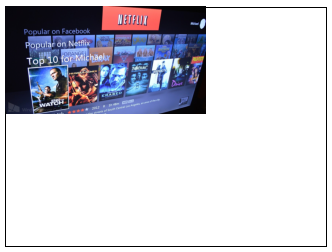
\includegraphics[width=\paperwidth]{general_figures/ml_intro_1}}}
\only<2>{\makebox[\linewidth]{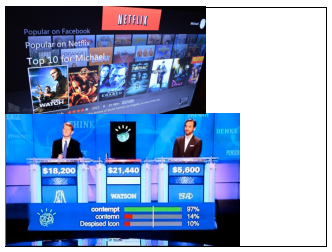
\includegraphics[width=\paperwidth]{general_figures/ml_intro_2}}}
\only<3>{\makebox[\linewidth]{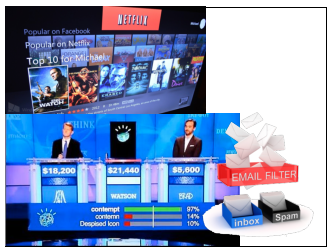
\includegraphics[width=\paperwidth]{general_figures/ml_intro_3}}}
\only<4>{\makebox[\linewidth]{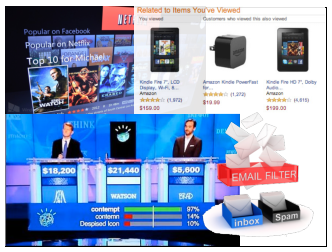
\includegraphics[width=\paperwidth]{general_figures/ml_intro_4}}}
\only<5>{\makebox[\linewidth]{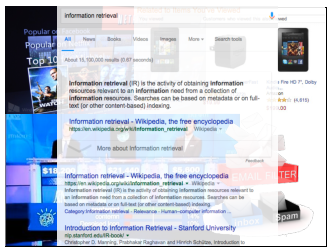
\includegraphics[width=\paperwidth]{general_figures/ml_intro_5}}}
\only<6->{\makebox[\linewidth]{
\includegraphics[width=\paperwidth]{general_figures/blackbox}}}
\only<7>{

\vspace{-5cm}
\begin{block}{Takeaways}
  \begin{itemize}
    \item ML should be interpretable
    \item We should measure interpretability
    \item Interpretability should reflect the world we want
  \end{itemize}
\end{block}

}
\end{frame}


\begin{frame}
\frametitle{The Challenge of Big Data}

\begin{columns}

\column{.5\linewidth}

Every second \dots
\begin{itemize}
  \item 600 new blog posts appear
  \item 34,000 tweets are tweeted
  \item 30 GB of data uploaded to Facebook
\end{itemize}
\pause

\begin{block}{Unstructured}
  No XML, no semantic web, no annotation.  Often just raw text.
\end{block}

\column{.5\linewidth}

\only<3->{
Common task: what's going on in this dataset.
\begin{itemize}
   \item Intelligence analysts
   \item Brand monitoring
   \item Journalists
   \item Humanists
\end{itemize}
}
\only<4>{
\centering
Common solution: unsupervised machine learning (topic models)
}

\end{columns}

\end{frame}

\begin{frame}

\begin{center}
\frametitle{What does a Topic Model do?}
From an \textbf<1>{input corpus} and number of topics \textbf<1>{$K$} $\rightarrow$ \textbf<2>{words to topics} \\
\only<1>{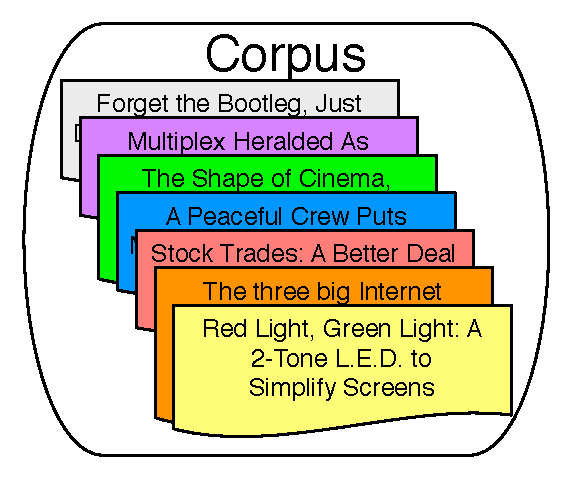
\includegraphics[width=0.6\linewidth]{reading_tea_leaves/figures/heldout_0} }
\only<2>{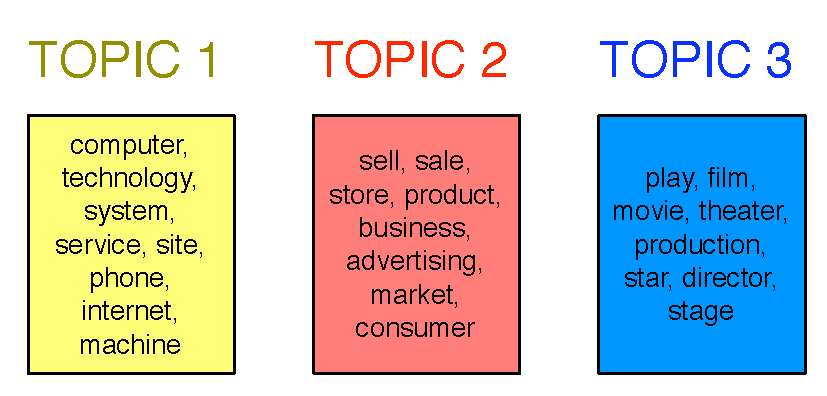
\includegraphics[width=0.9\linewidth]{reading_tea_leaves/figures/nyt_topics_wide}}
%\only<3>{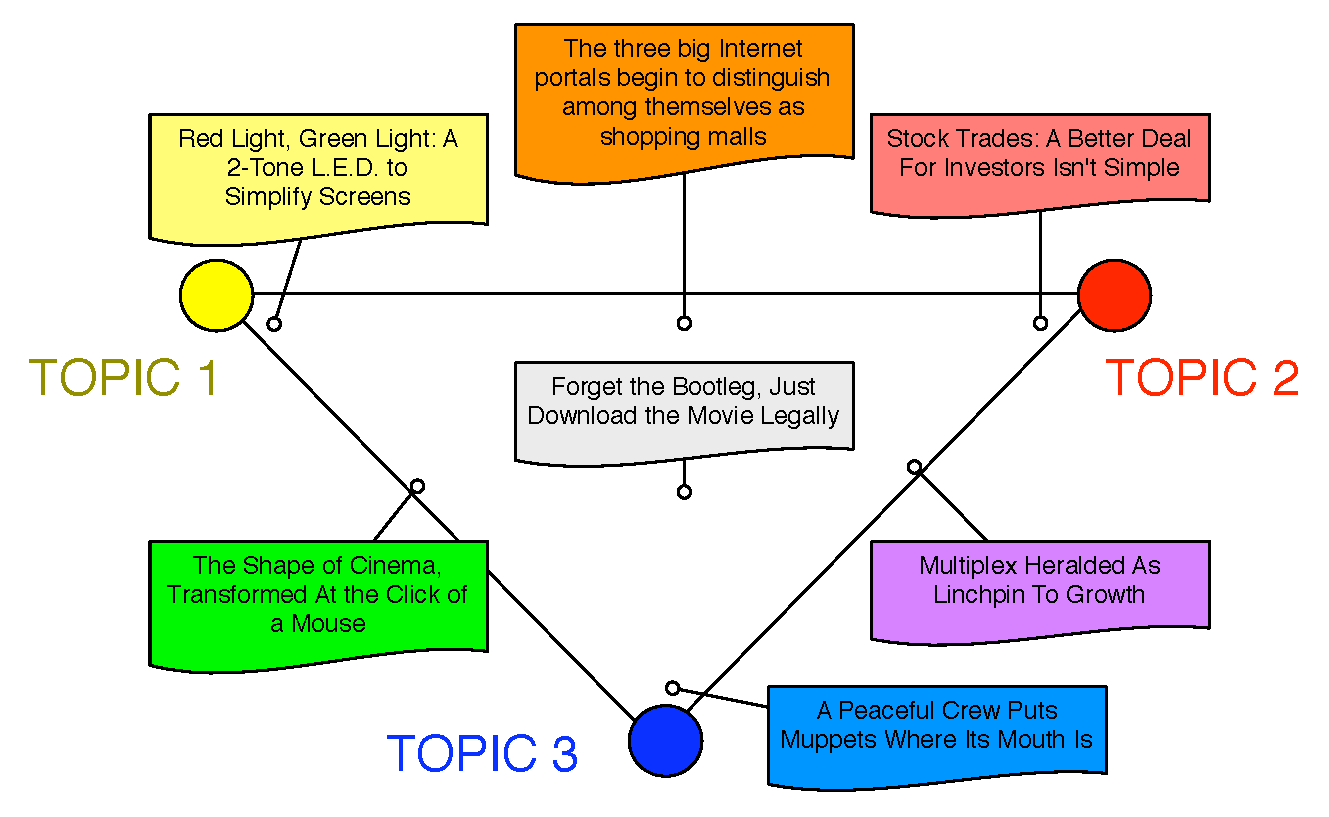
\includegraphics[width=0.9\linewidth]{topic_models/nyt_documents}}
\end{center}

\end{frame}


\begin{frame}{Evaluating Topic Models}

\begin{columns}

\column{.6\linewidth}
\begin{block}{ Reading Tea Leaves: How Humans Interpret Topic Models}
Jonathan Chang, Jordan Boyd-Graber, Chong Wang, Sean Gerrish, and David
M. Blei. Reading Tea Leaves: How Humans Interpret Topic Models. Neural
Information Processing Systems, 2009.
\end{block}

\column{.3\linewidth}
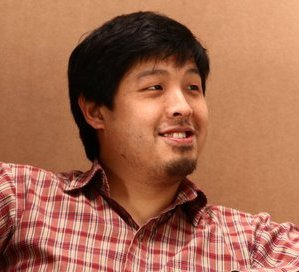
\includegraphics[width=.8\linewidth]{general_figures/jonathan}

\end{columns}

\end{frame}



\frame{
\frametitle{Evaluation}
\begin{center}
%\only<1>{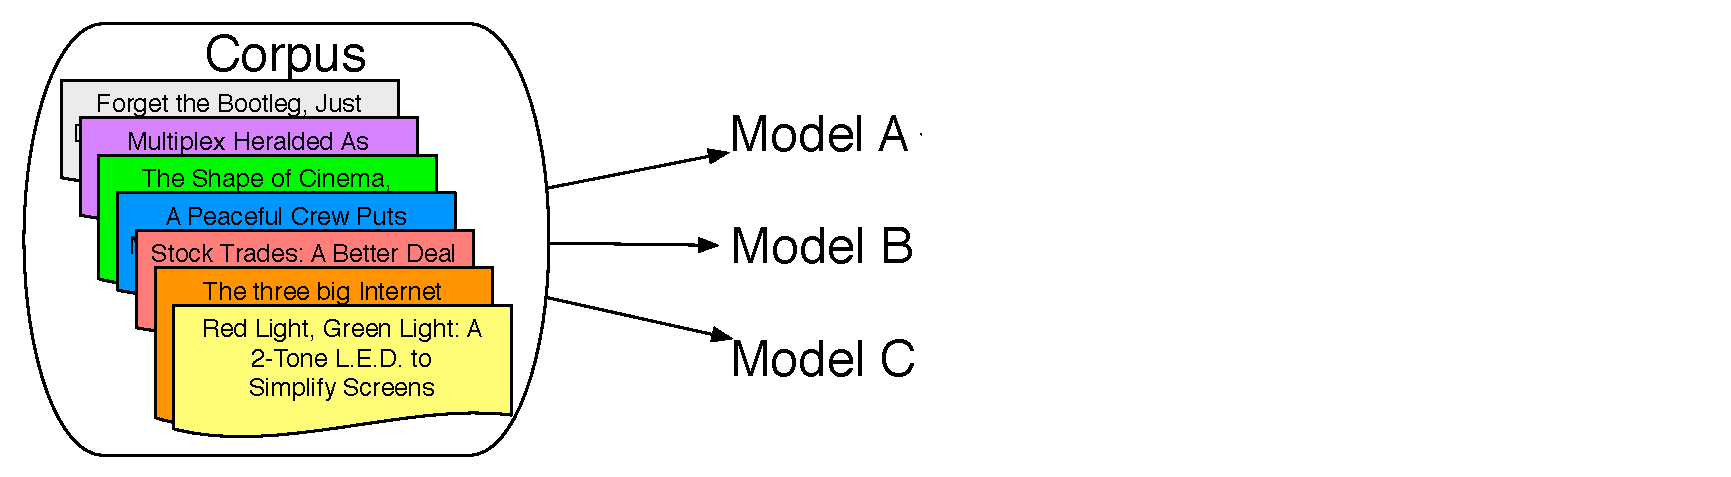
\includegraphics[width=0.9\linewidth]{reading_tea_leaves/figures/heldout_1} }
\only<1>{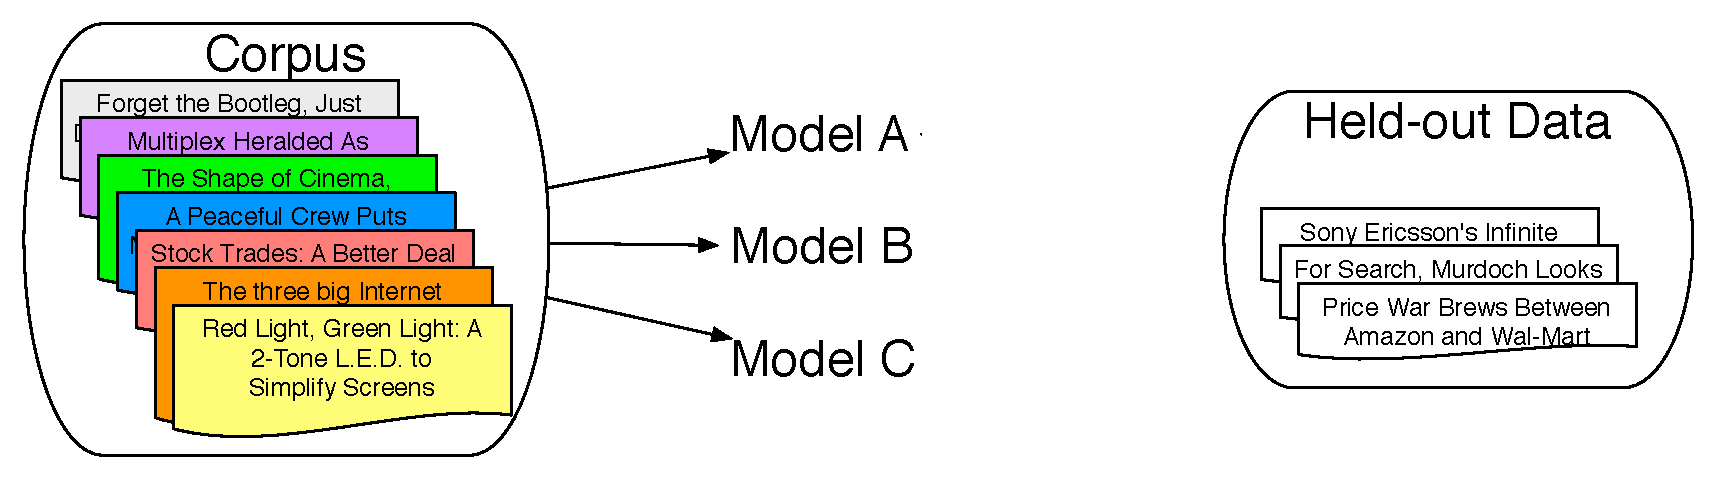
\includegraphics[width=\linewidth]{reading_tea_leaves/figures/heldout_2} }
%\only<3>{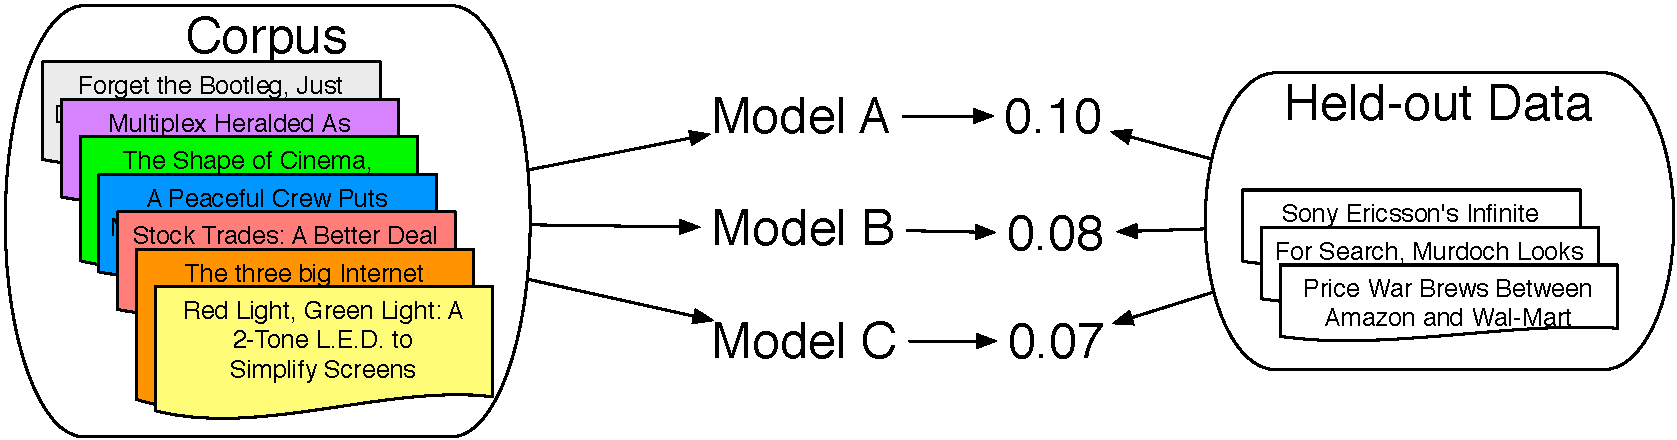
\includegraphics[width=\linewidth]{reading_tea_leaves/figures/heldout_3} }
\only<2>{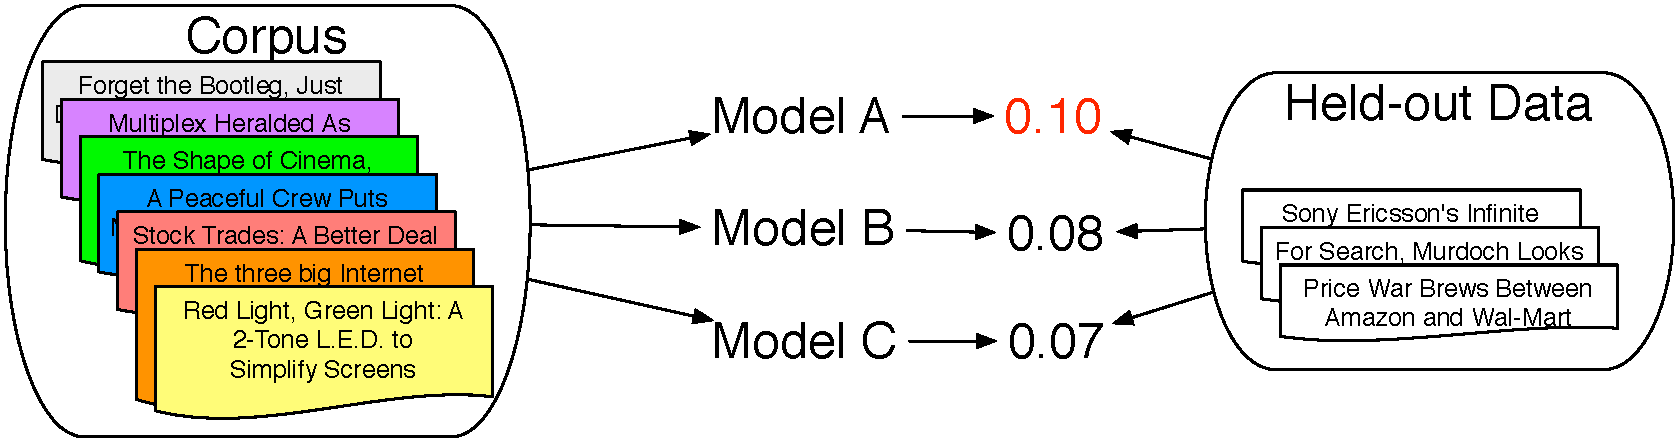
\includegraphics[width=\linewidth]{reading_tea_leaves/figures/heldout_4}  \\
	\large Measures predictive power (likelihood)}
\end{center}
}

\begin{frame}{But we don't use topic models for prediction!}

\gfxs{autocomplete}{.8}

\end{frame}

\frame{
\frametitle{Qualitative Evaluation of the Latent Space}

\begin{center}
\only<1>{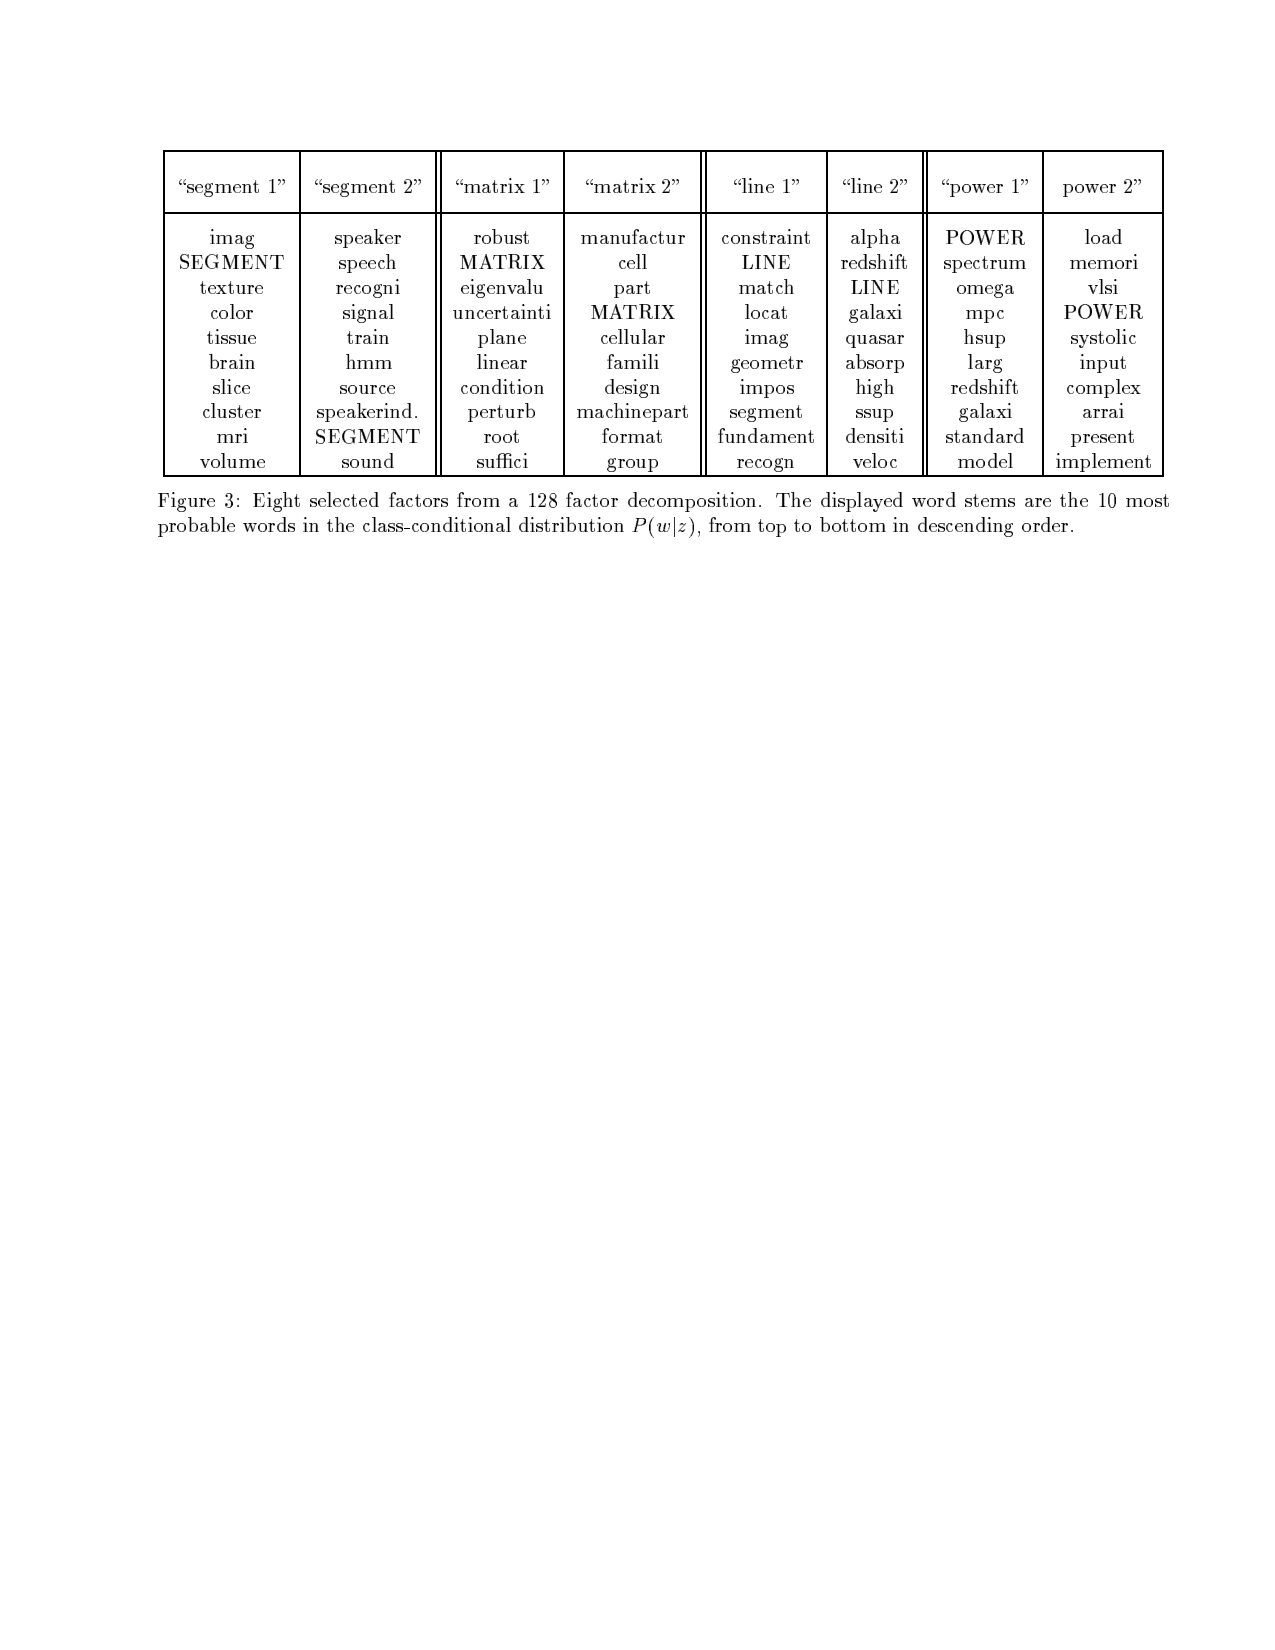
\includegraphics[width=0.9\linewidth]{reading_tea_leaves/topics_from_papers/1} \\ \cite{hofmann-99} }
\only<2>{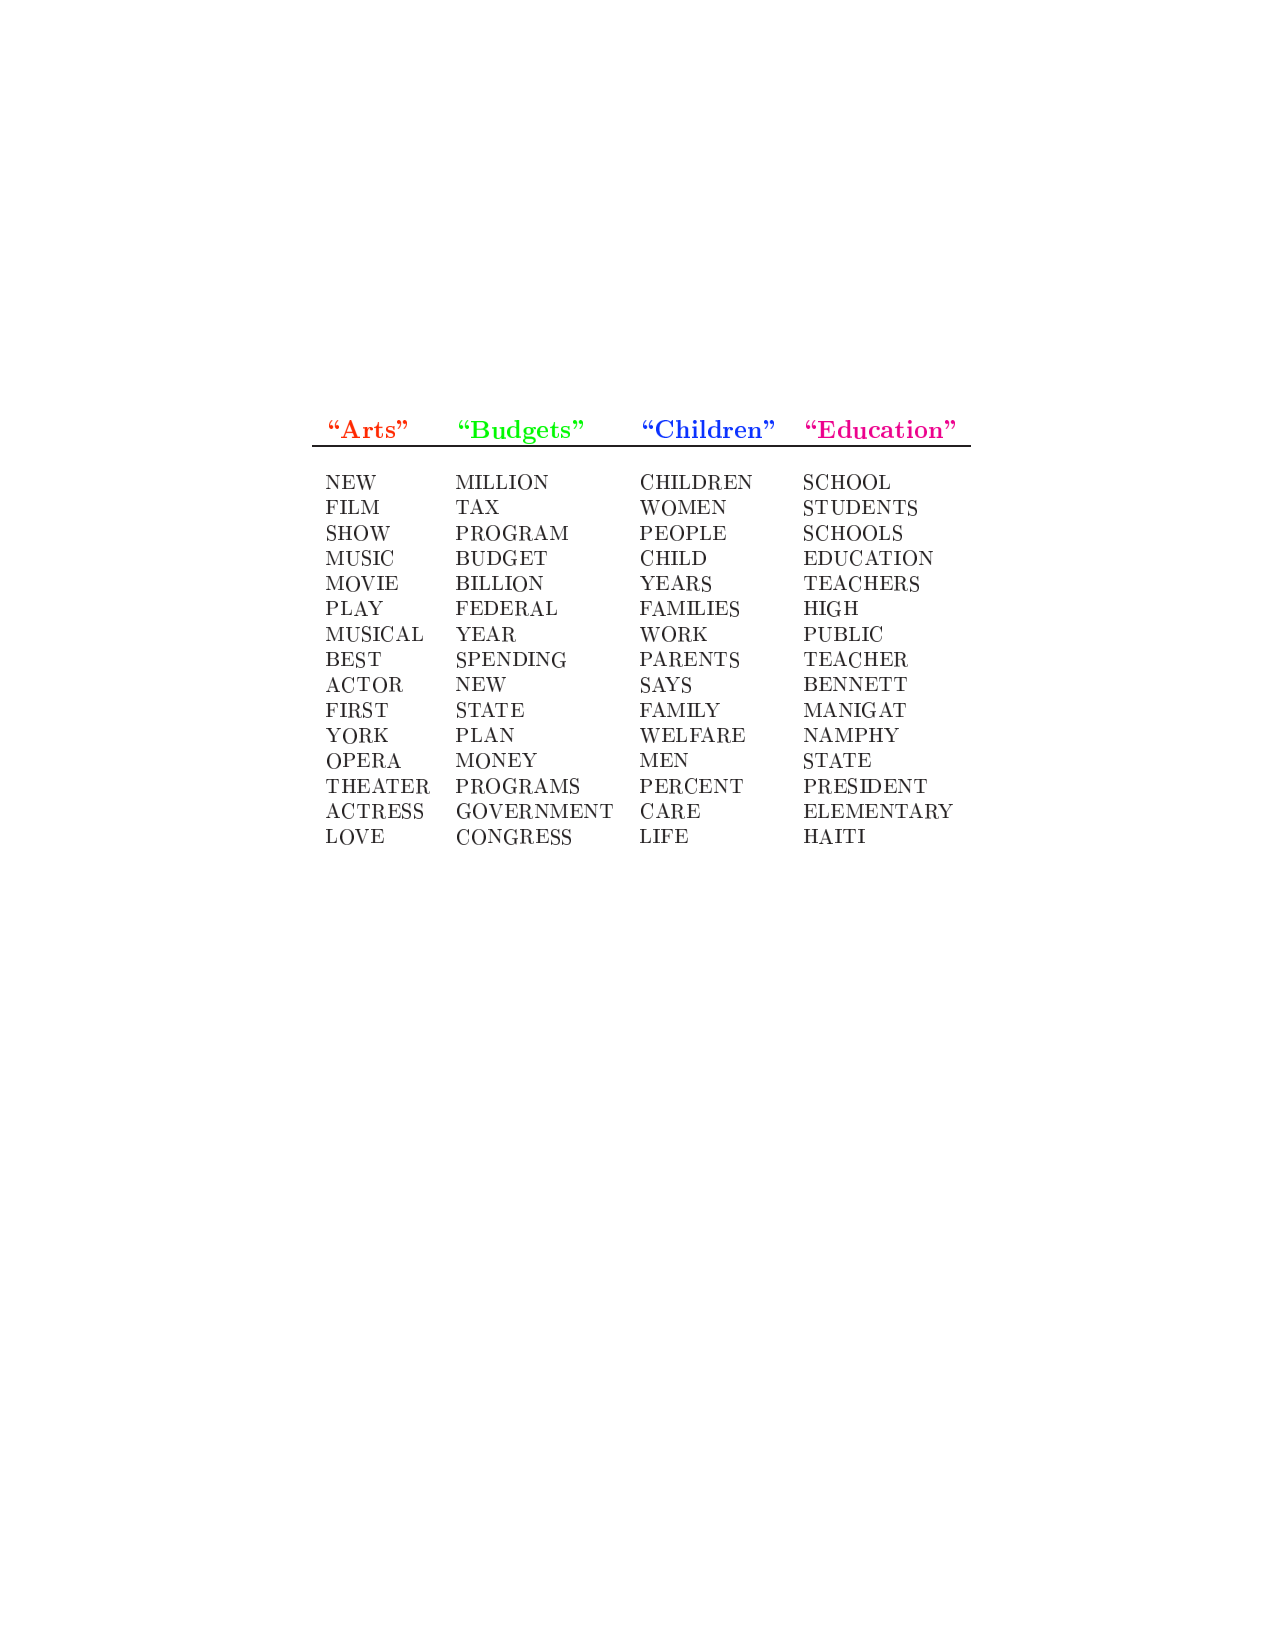
\includegraphics[width=0.7\linewidth]{reading_tea_leaves/topics_from_papers/2} \\ \cite{blei-03} }
\only<3>{
\includegraphics[width=0.7\linewidth]{reading_tea_leaves/topics_from_papers/3} \\ \cite{mimno-09} }
\only<4>{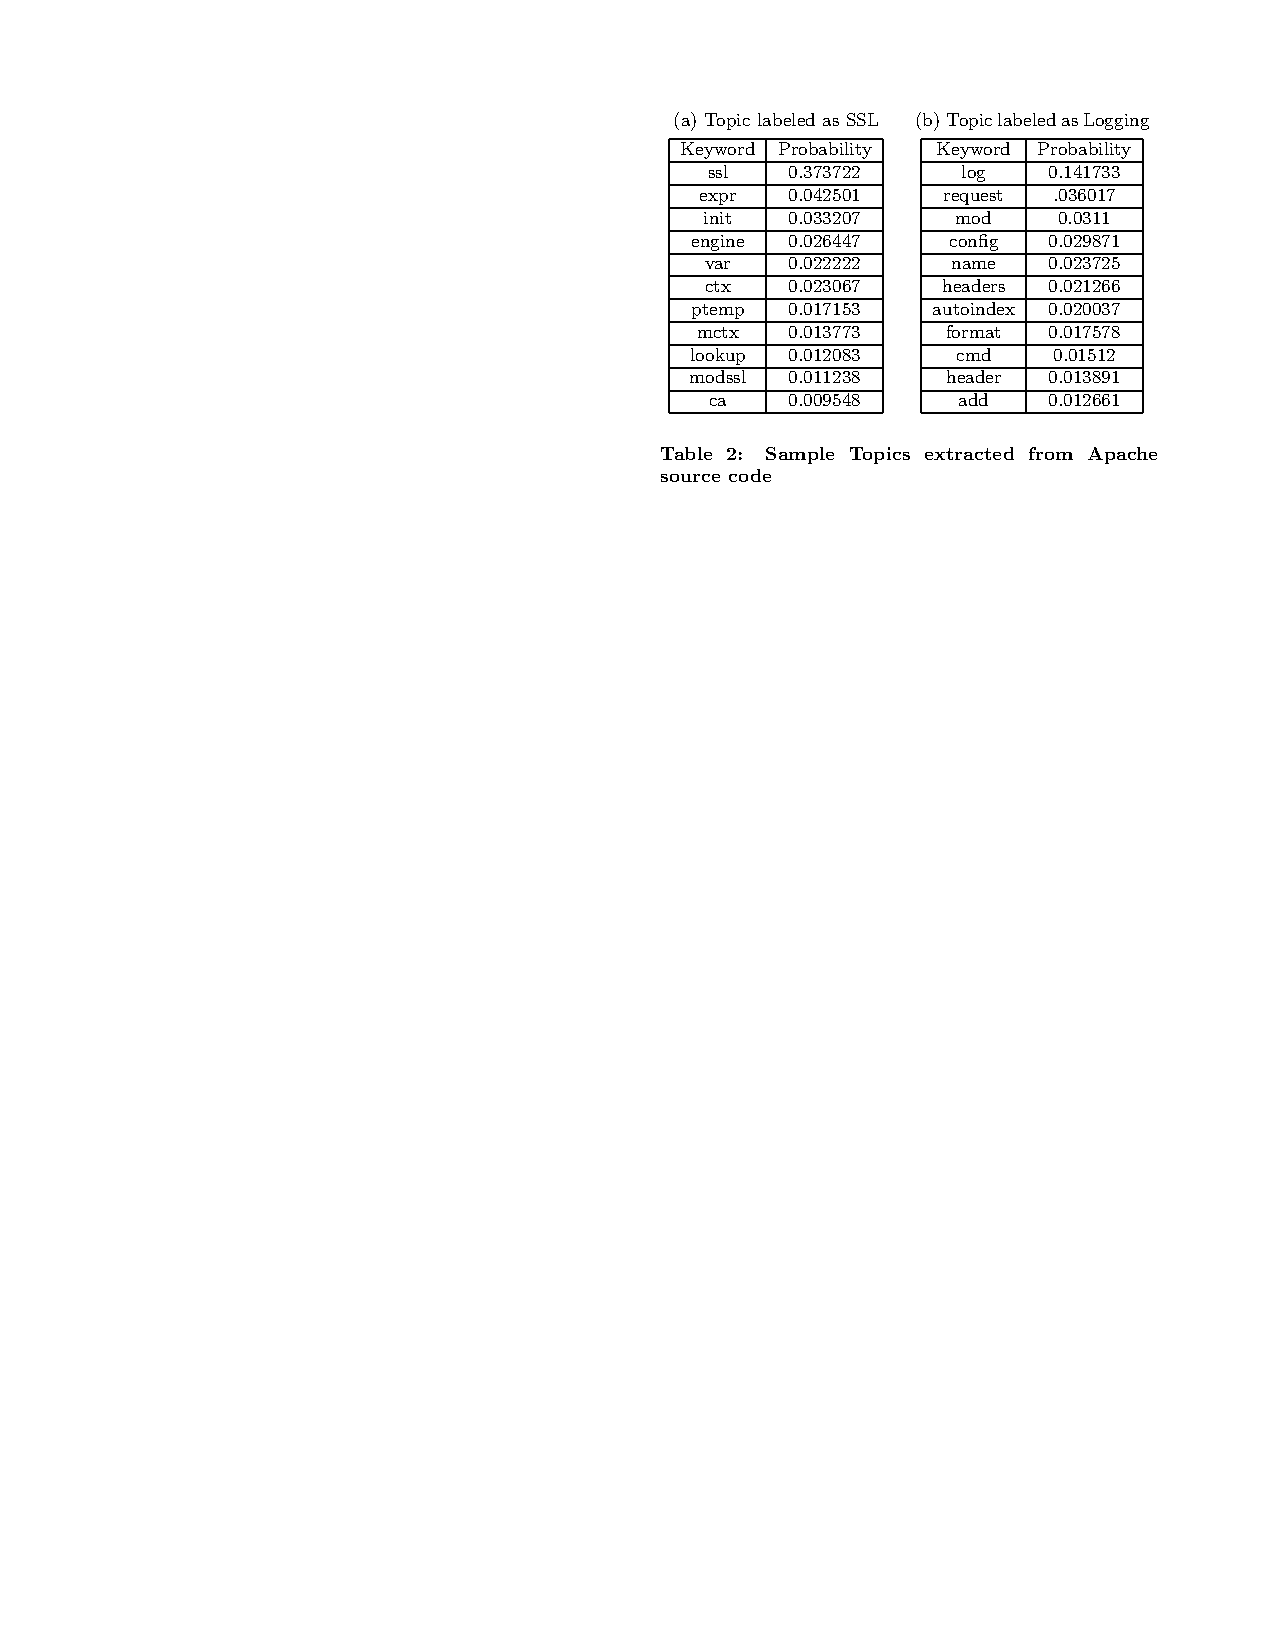
\includegraphics[width=0.7\linewidth]{reading_tea_leaves/topics_from_papers/4}
  \\ \cite{maskeri-08} }
\end{center}
}

\frame{
  \frametitle{Word Intrusion}

  \begin{itemize}
    \item Take the highest probability words from a topic

      \begin{block}{Original Topic}
        dog \\ cat \\ \only<2->{\alert<2->{apple} \\ } horse \\ pig \\ cow
      \end{block}

\only<2->{    \item \alert<2>{Intruder: high probability word from another topic}}
\pause
  \end{itemize}
}

\frame{
\frametitle{Interpretability and Likelihood}


\begin{center}
\only<1>{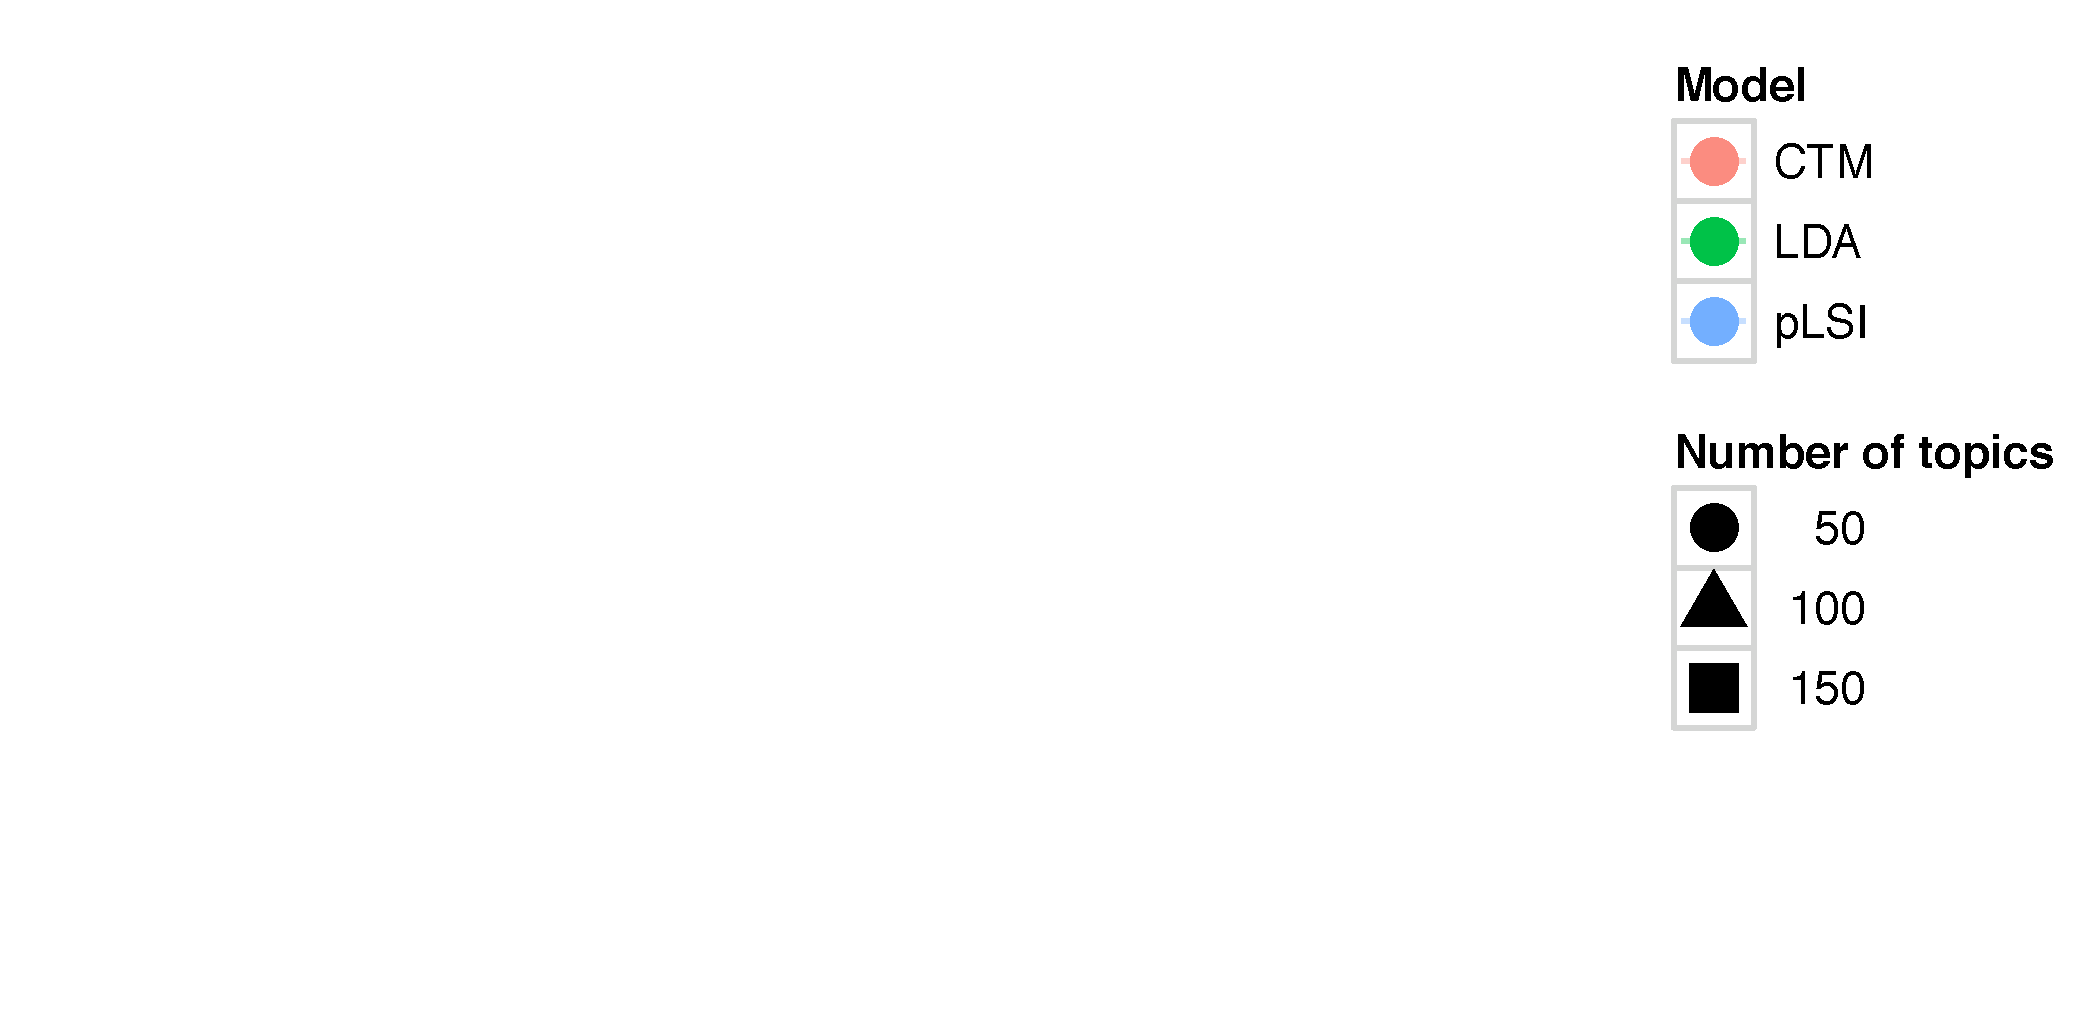
\includegraphics[width=.8\paperwidth]{reading_tea_leaves/figures/prec_ll_1}}
\only<2>{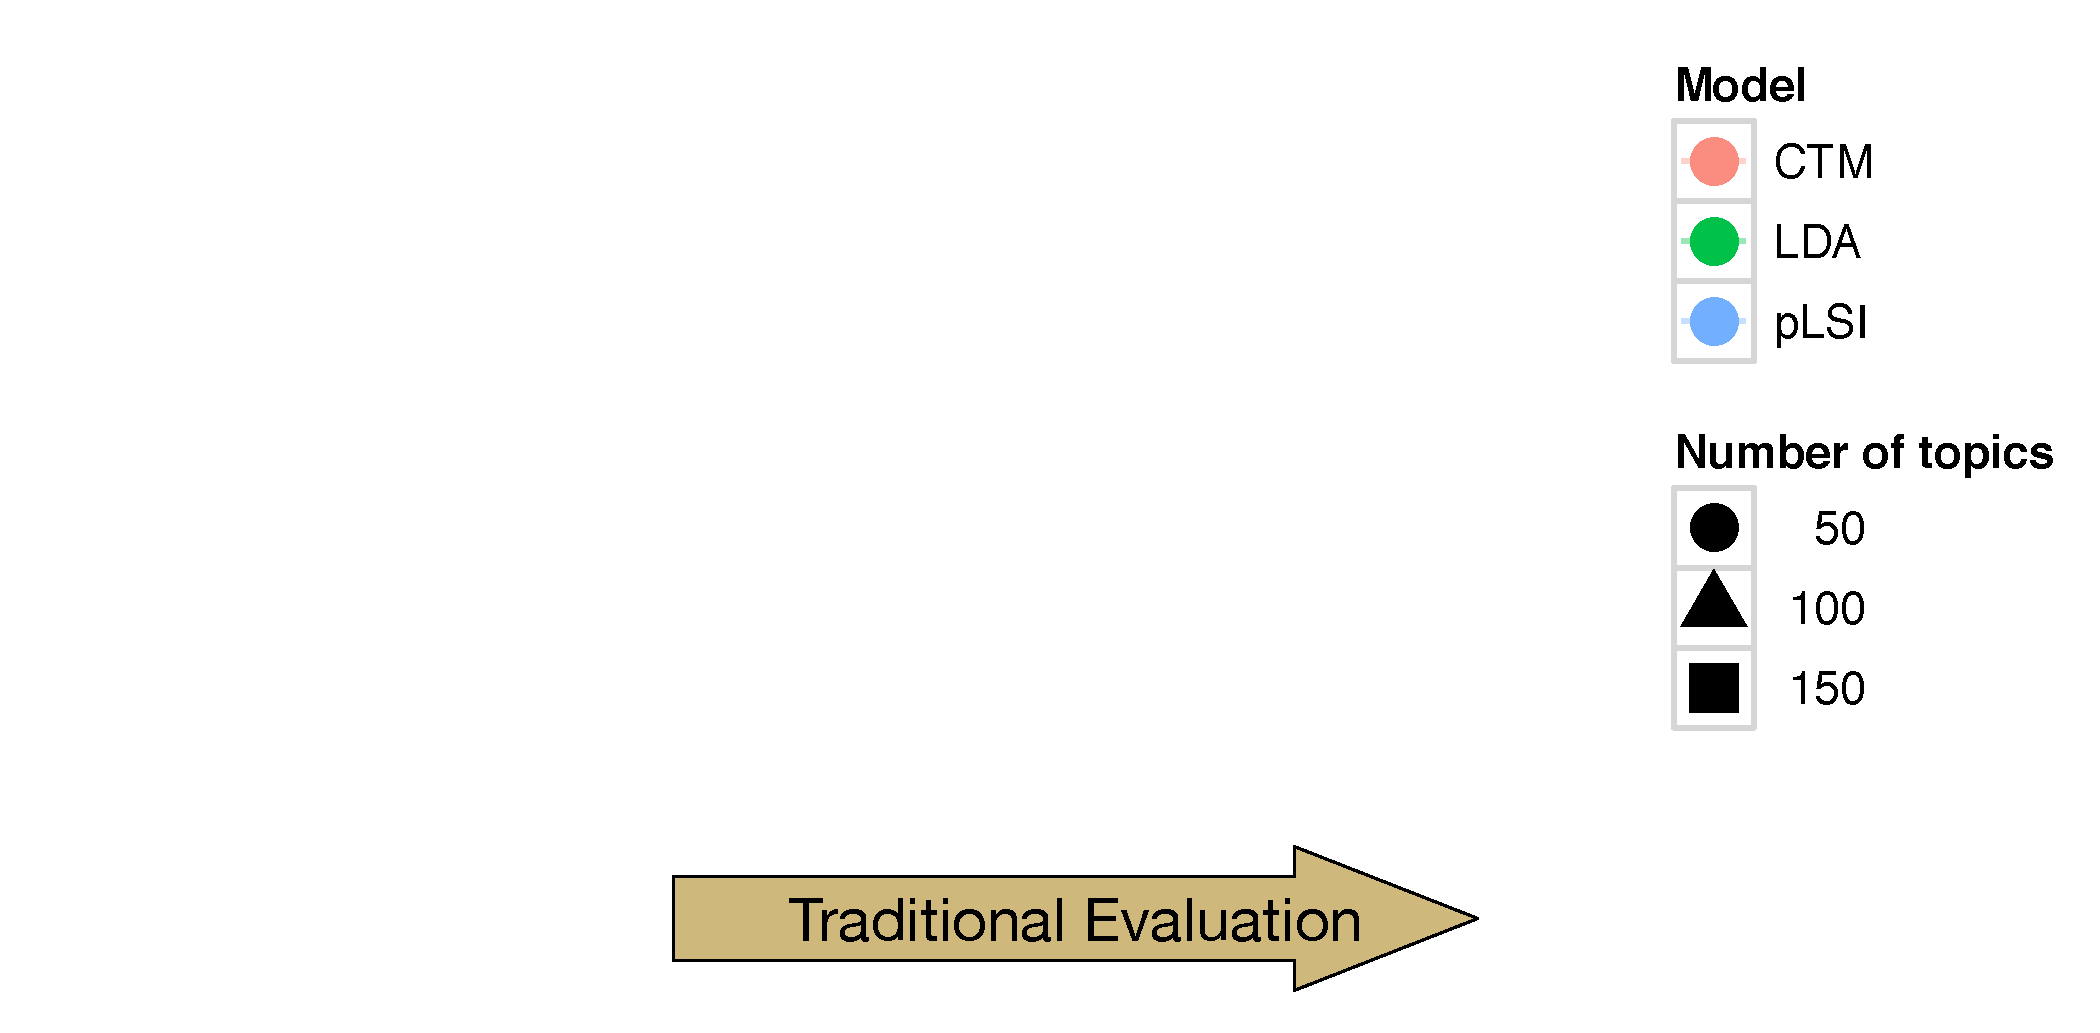
\includegraphics[width=.8\paperwidth]{reading_tea_leaves/figures/prec_ll_2}}
\only<3>{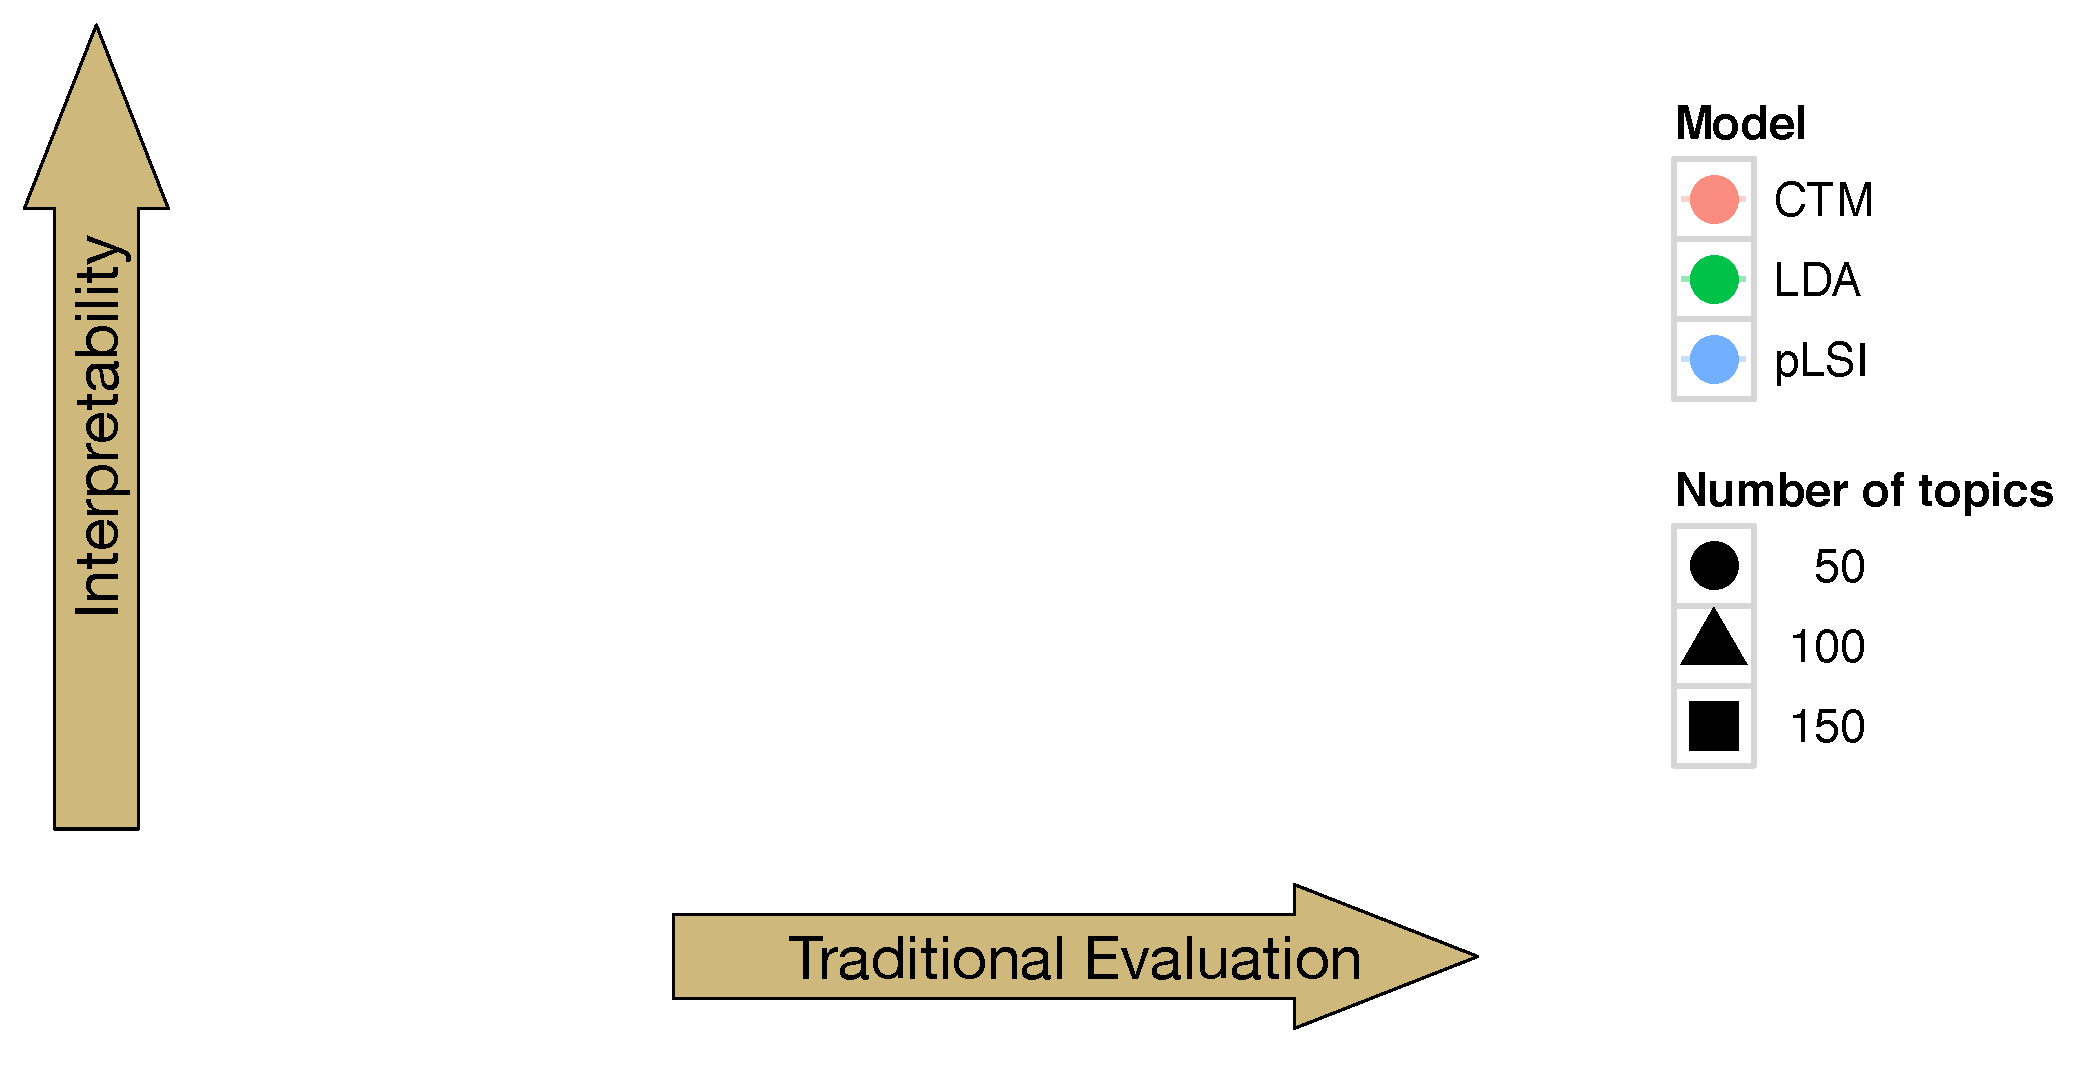
\includegraphics[width=.8\paperwidth]{reading_tea_leaves/figures/prec_ll_3}}
\only<4>{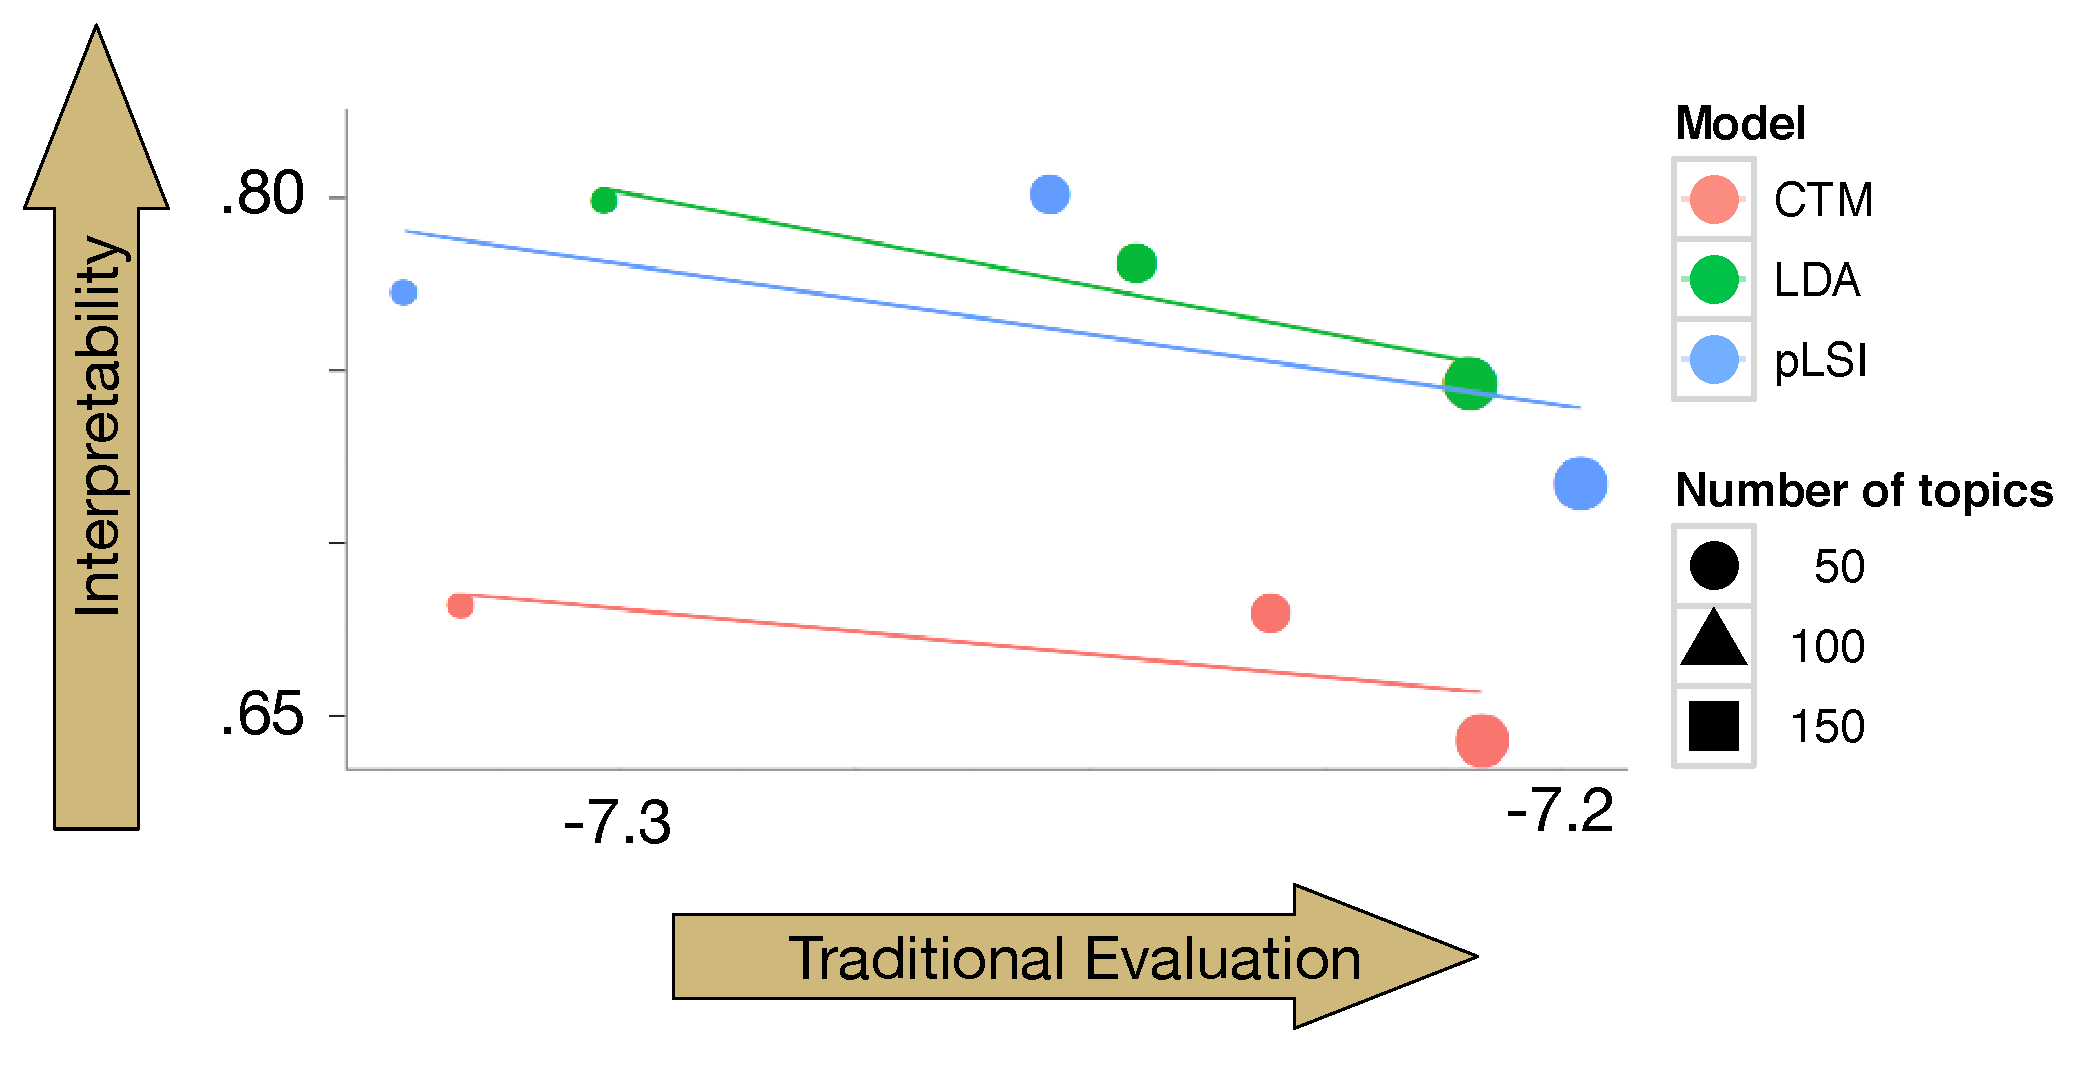
\includegraphics[width=.8\paperwidth]{reading_tea_leaves/figures/prec_ll_4}}
\only<4>{\\ Within a model, higher likelihood $\not =$ higher interpretability}
\end{center}
}


\begin{frame}{Since then \dots}

  \begin{itemize}
    \item A way to get at an evaluation that matches {\bf what we care about}
    \item A necessary step to improving topic models for navigating large datasets~\cite{talley-11}
    \item Others have discovered automatic methods that uncover the same properties~\cite{newman-10,mimno-11}
    \item And extended the technique to structured topics and
      phrases~\cite{lindsey-12,weninger-12}
    \item \alert<2>{Extending to multiple users}~\cite{Felt-15}
      \ifjobtalk (CoNLL Best Paper) \fi
  \end{itemize}

\end{frame}


\begin{frame}
\frametitle{The Problem: User Perspective}

\begin{columns}

\column{.4\linewidth}
\begin{center}
\begin{tabular}{ccc}
& \only<2->{\itmspace}\color<2->{red}{bladder} & \\
& \only<3->{\hspace{-2cm}} \color<3->{blue}{spinal\_cord}  & \\
& \only<3->{\hspace{-2cm}} \color<3->{blue}{sci} & \\
& \only<3->{\hspace{-2cm}}\color<3->{blue}{spinal\_cord\_injury} & \\
& \only<3->{\hspace{-2cm}}\color<3->{blue}{spinal} & \\
& \only<2->{\itmspace}\color<2->{red}{urinary} & \\
& \only<2->{\itmspace}\color<2->{red}{urothelial} & \\
& \only<3->{\hspace{-2cm}}\color<3->{blue}{cervical} & \\
& injury & \\
& recovery & \\
& \only<2->{\itmspace}\color<2->{red}{urinary\_tract} & \\
& locomotor & \\
& \only<3->{\hspace{-2cm}}\color<3->{blue}{lumbar} & \\
\end{tabular}
\end{center}

\column{.6\linewidth}

\danquote{These words don't belong together!}

\end{columns}

\end{frame}


\frame{

\begin{columns}

\column{.5\linewidth}

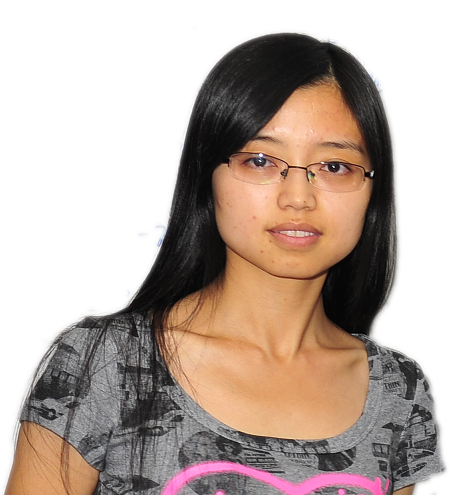
\includegraphics[width=.8\linewidth]{general_figures/yuening}

\column{.5\linewidth}

\begin{block}{Interactive Topic Modeling}
Yuening Hu, Jordan Boyd-Graber, and Brianna Satinoff.  Association for Computational Linguistics, 2011.
\end{block}


\end{columns}

}



\frame{
	\frametitle{How to fix it?}


	\only<1>{	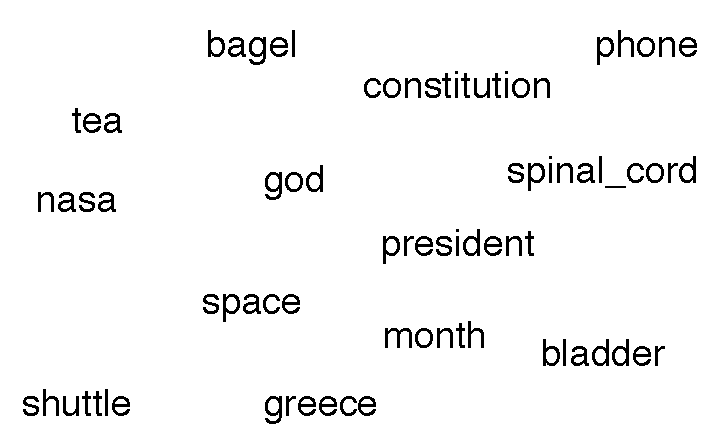
\includegraphics[width=\linewidth]{interactive_topic_models/constraints_1}     }
	\only<2>{	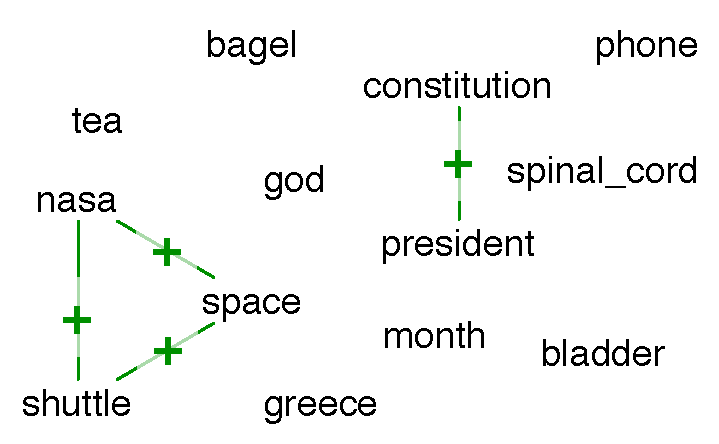
\includegraphics[width=\linewidth]{interactive_topic_models/constraints_2}     }
	\only<3>{	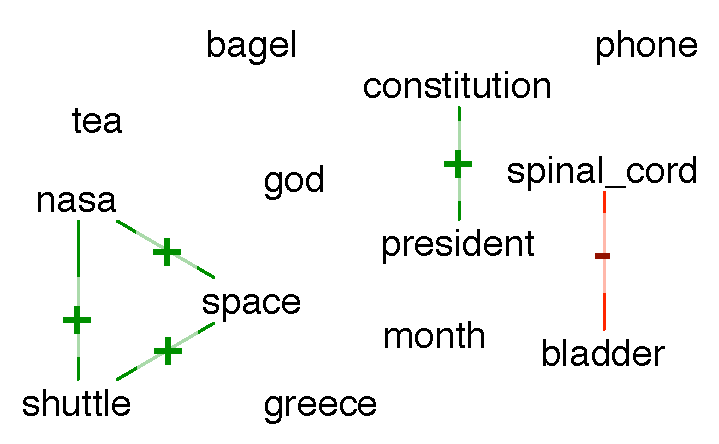
\includegraphics[width=\linewidth]{interactive_topic_models/constraints_3}     }


}


\providecommand{\tb}[1]{\parbox{0.8\linewidth}{ \tiny{ #1 }} \vspace{.2cm} }

\frame{

\vspace{-1cm}

\begin{columns}

\column{.5\linewidth}

\begin{tabular}{l*{2}{c}r}
	Topic & Before \\
\hline

\alert<2>{{\bf 1}} & \tb{ \alert<2>{election, yeltsin, russian, political, party, democratic, russia,
  president, democracy, boris, country, south, years, month, government, vote,
  since, leader, presidential, military} } \\

2 & \tb{new, york, city, state, mayor, budget, giuliani, council, cuomo, gov,
  plan, year, rudolph, dinkins, lead, need, governor, legislature, pataki,
  david} \\

3 & \tb{nuclear, arms, weapon, defense, treaty, missile, world, unite, yet,
  soviet, lead, secretary, would, control, korea, intelligence, test, nation,
  country, testing} \\

4 & \tb{president, bush, administration, clinton, american, force, reagan, war,
  unite, lead, economic, iraq, congress, america, iraqi, policy, aid,
  international, military, see} \\

& \vdots \\

\alert<2>{{\bf 20}} & \tb{\alert<2>{soviet, lead, gorbachev, union, west, mikhail, reform, change, europe,
  leaders, poland, communist, know, old, right, human, washington, western,
  bring, party} }\\

\end{tabular}

\column{.5\linewidth}

\only<3> {

	\begin{block}{Suggestion}
	\emph{boris, communist, gorbachev, mikhail, russia,
  russian, soviet, union, yeltsin }
	\end{block}

}

\only<4-> {

\begin{tabular}{l*{2}{c}r}
	Topic & After \\
\hline

\alert<5>{{\bf 1}} & \alert<5>{\tb{election, democratic, south, country, president, party, africa, lead,
  even, democracy, leader, presidential, week, politics, minister, percent,
  voter, last, month, years} } \\

\alert<6>{2} & \tb{new, york, city, state, mayor, budget, council, giuliani, gov, cuomo,
  year, rudolph, dinkins, legislature, plan, david, governor, pataki, need, cut}
\\

\alert<6>{3} & \tb{nuclear, arms, weapon, treaty, defense, war, missile, may, come, test,
  american, world, would, need, lead, get, join, yet, clinton, nation} \\

\alert<6>{4} & \tb{president, administration, bush, clinton, war, unite, force, reagan,
  american, america, make, nation, military, iraq, iraqi, troops, international,
  country, yesterday, plan} \\

   & \vdots \\

\alert<4>{ {\bf 20} } & \alert<4> {\tb{soviet, union, economic, reform, yeltsin, russian, lead, russia,
  gorbachev, leaders, west, president, boris, moscow, europe, poland, mikhail,
  communist, power, relations} } \\

\end{tabular}

}

\end{columns}

}


\providecommand{\blue}[1]{{\color{blue}{#1}}}
\providecommand{\red}[1]{{\color{red}{#1}}}
\providecommand{\green}[1]{{\color{green}{#1}}}

\begin{frame}

\frametitle{Example: Negative Constraint}

\begin{columns}

\column{.4\linewidth}

\begin{tabular}{l*{2}{c}r}
	Topic & Words \\
\hline

{\bf 318} & \tb{\red{bladder}, sci, \blue{spinal\_cord}, \blue{spinal\_cord\_injury}, \blue{spinal}, \red{urinary}, \red{urinary\_tract}, \red{urothelial},\blue{injury}, \blue{motor}, \blue{recovery}, \blue{reflex}, \blue{cervical}, \red{urothelium}, \blue{functional\_recovery}} \\

\end{tabular}

\column{.1\linewidth}

\column{.4\linewidth}

\only<3->{
\begin{tabular}{l*{2}{c}r}
	Topic & Words \\
\hline

{\bf 318} & \tb{sci, \blue{spinal\_cord}, \blue{spinal\_cord\_injury}, \blue{spinal}, \blue{injury}, \blue{recovery}, \blue{motor}, \blue{reflex}, \red{urothelial}, \green{injured}, \blue{functional\_recovery}, \green{plasticity}, \green{locomotor}, \blue{cervical}, \green{locomotion}}\\

\end{tabular}
}

\end{columns}

\only<2->{
\begin{block}{Negative Constraint}
  spinal\_cord, bladder
\end{block}

}

\end{frame}




\begin{frame}{Task-Based Metrics}

\begin{center}
  \only<1>{  
\includegraphics[width=.9\paperwidth]{interpretability/lime_fe_cartoon_1}
  }
  \only<2>{  
\includegraphics[width=.9\paperwidth]{interpretability/lime_fe_cartoon_2}
  }
  \only<3>{  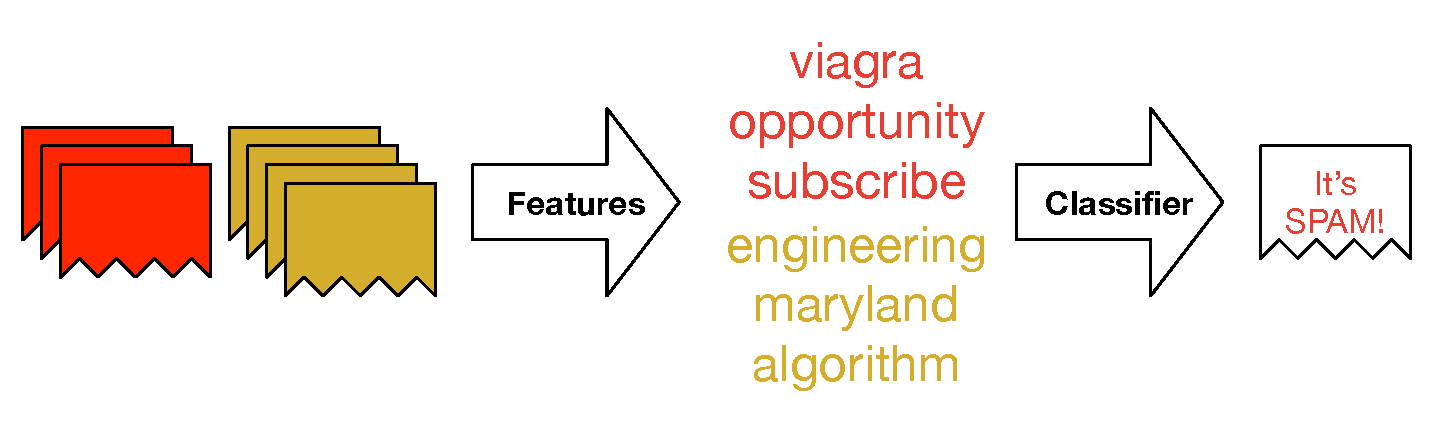
\includegraphics[width=.9\paperwidth]{interpretability/lime_fe_cartoon_3}  }
\end{center}

\end{frame}

\begin{frame}{LIME}

  \gfxi{lime_local}{.7}

Marco Tulio Ribeiro, Sameer Singh, and Carlos Guestrin.  ``Why Should
I Trust You?'' Explaining the Predictions of Any Classifier.  KDD
2016. \\

LIME: Local Interpretable Model-Agnostic Explanations

\end{frame}


\begin{frame}{Improving ML Algorithms}

  \only<1>{  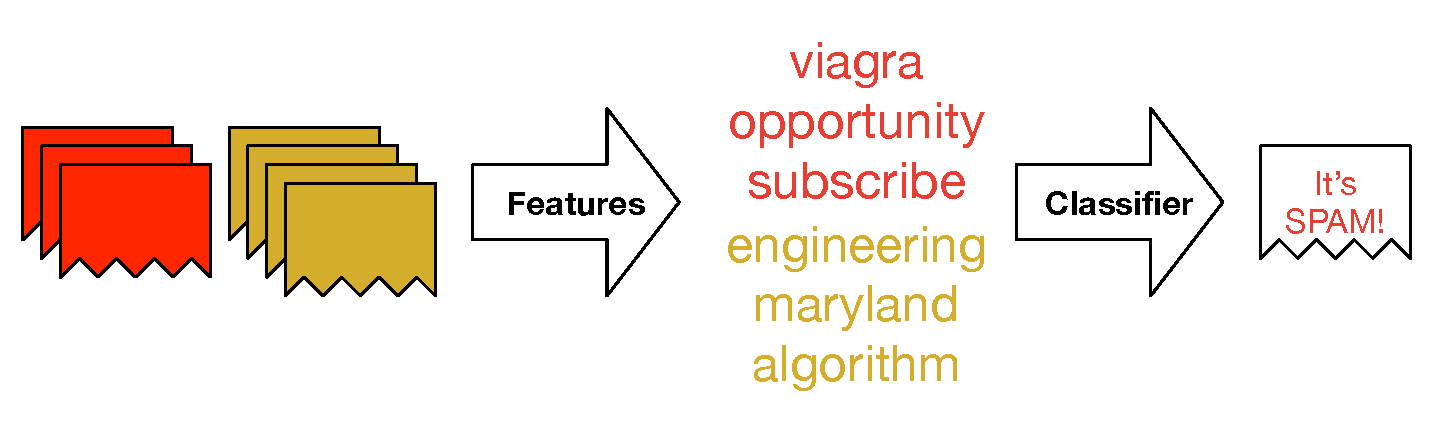
\includegraphics[width=.9\paperwidth]{interpretability/lime_fe_cartoon_3}
  }
  \only<2>{  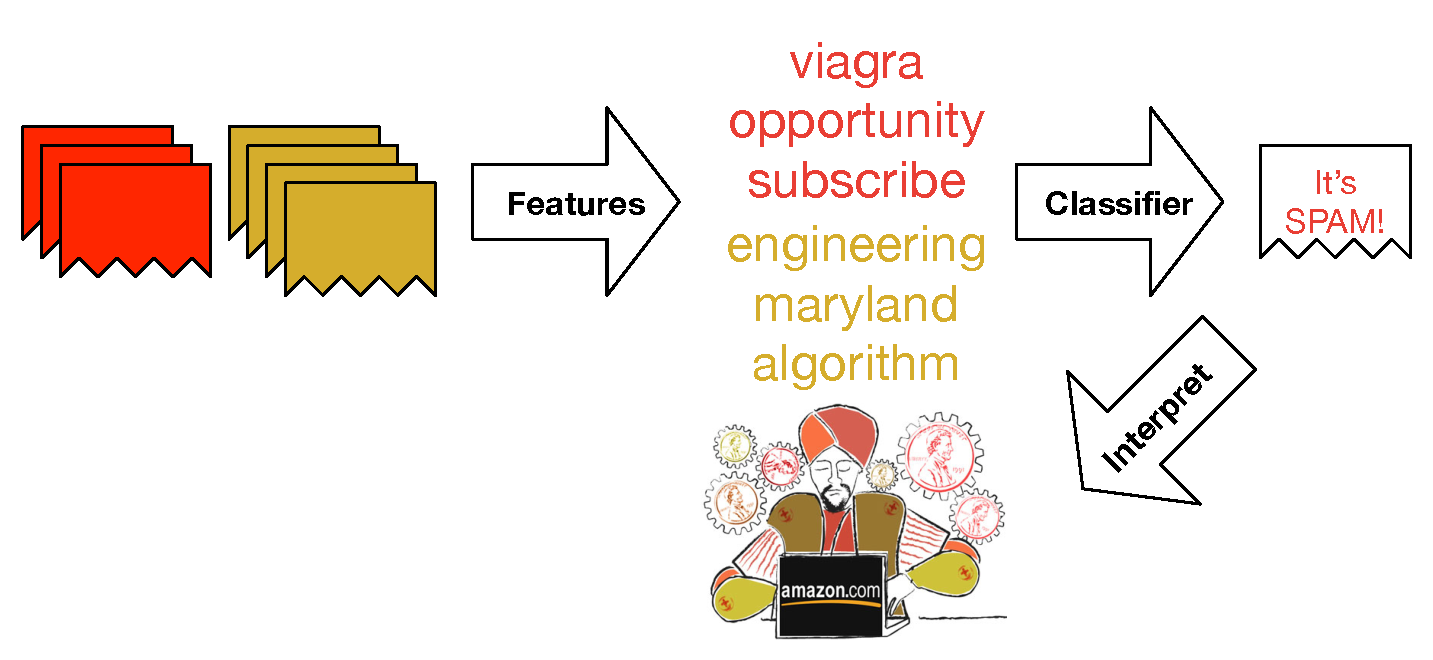
\includegraphics[width=.9\paperwidth]{interpretability/lime_fe_cartoon_4}
  }
  \only<3>{  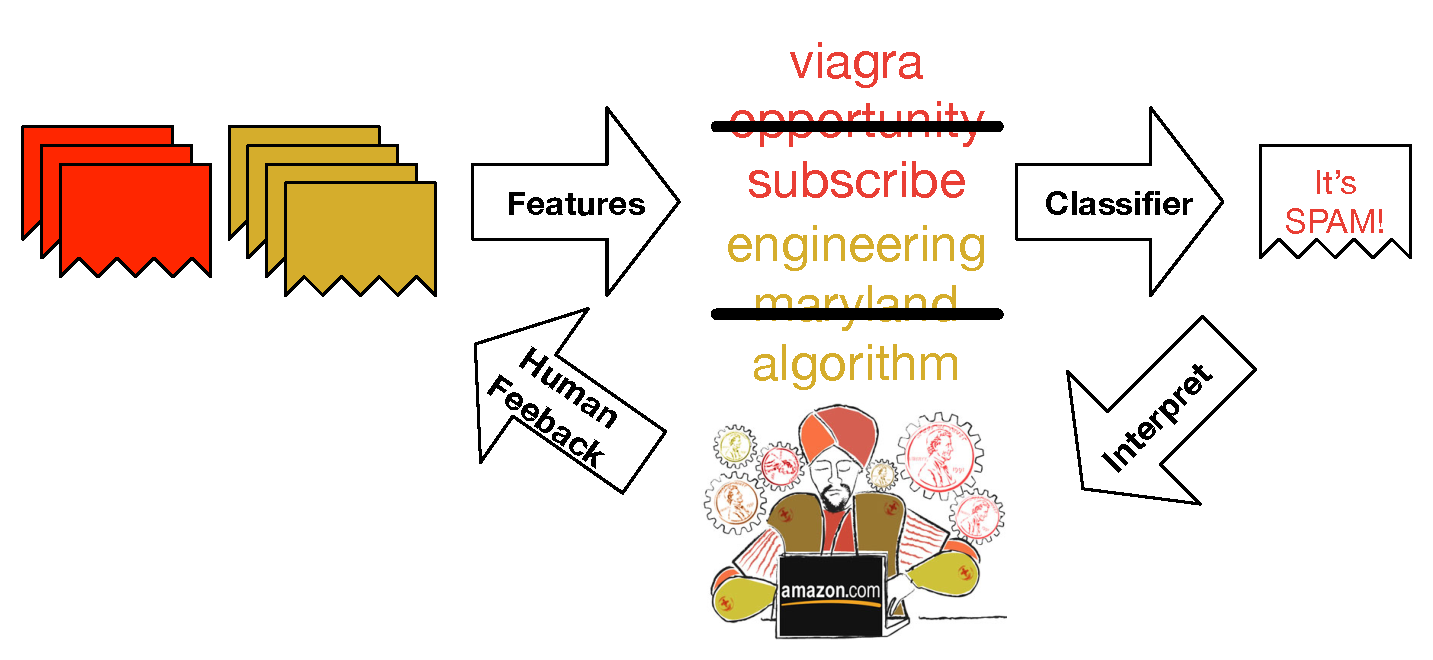
\includegraphics[width=.9\paperwidth]{interpretability/lime_fe_cartoon_5}  }
  \only<4>{  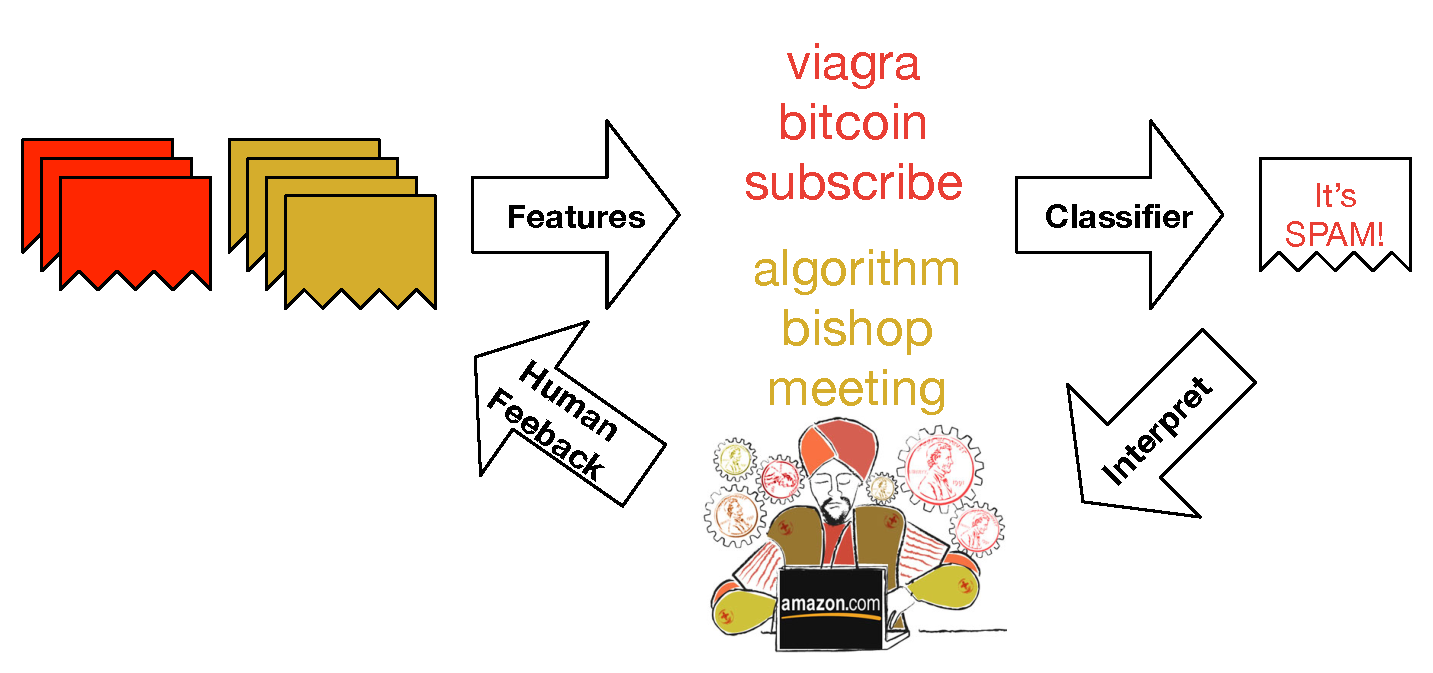
\includegraphics[width=.9\paperwidth]{interpretability/lime_fe_cartoon_6}
  }

  \only<5>{\gfxi{mt_task}{1.0}}
  \only<6>{\gfxi{mt_results}{1.0}}
\end{frame}

\fsi{general_figures/kill_all_humans}{}
\fsi{general_figures/enslave_humans}{}
\fsi{general_figures/tng_poker}{}

\fsi{qb/quizbowl}{}


% TODO add more questions here

\begin{frame}[t]
	\frametitle{Sample Question}

        The Swiss-Italian architect Pietro Antonio Solari
        \only<2->{built several fortified towers in this city, which
          often vied for power with its northern rival Tver. A ruler
          of this city prevailed in the} \only<3->{Great Stand on the
          Ugra River. A prince from this city was nicknamed for
          winning a battle on the} \only<4->{Don river. Partly because
          a ruler of this city married} \only<5->{Sophia Palaiologina,
          the niece of the last Byzantine Emperor, this city styled
          itself the} \only<6->{``Third Rome'' after the fall of
          Constantinople. Another prince of this city stopped paying
          tribute to the} \only<7->{Mongols in 1476, ending the
          ``Tatar yoke.''} \only<8->{The Grand Duchy headquartered in
          this city came to an end in 1547 with the ascension of}
        \only<9->{ Ivan IV, who made it his capital. For 10 points,
          name this city where Ivan III renovated the
          Kremlin,} \only<10->{the capital of Russia.}\\
        \vspace{.5cm} \only<11->{ {\bf Moscow} (Moskva / Muscovy)}



\end{frame}






\begin{frame}{}

  \begin{columns}
    \column{.4\linewidth}
        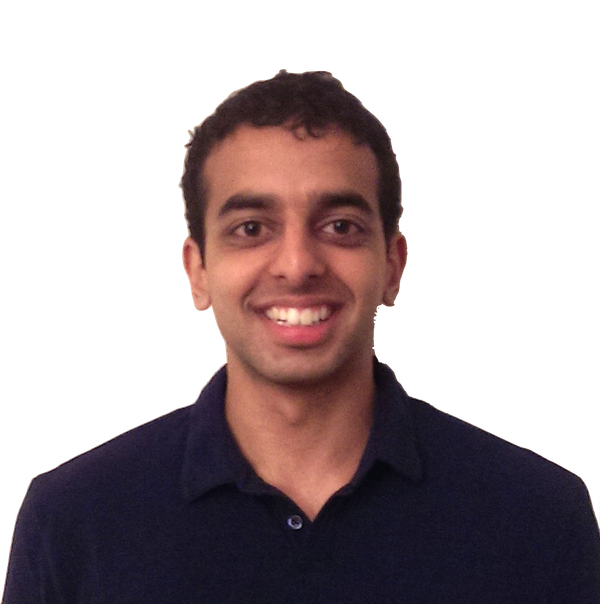
\includegraphics[width=0.7\linewidth]{general_figures/mohit}
    \column{.6\linewidth}
        \begin{block}{ {\bf \href{http://umiacs.umd.edu/~jbg//docs/2014_emnlp_qb_rnn.pdf}{A Neural Network for Factoid Question Answering over Paragraphs}}}
\underline{\href{http://cs.umd.edu/~miyyer/}{Mohit Iyyer}}, {\bf Jordan Boyd-Graber}, Leonardo Claudino, Richard Socher, and Hal {Daum\'{e} III}.  \emph{Empirical Methods in Natural Language Processing}, 2014
        \end{block}

        \begin{block}{ {\bf \href{file:///Users/jbg/public_html/docs/2015_acl_dan.pdf}{Deep Unordered Composition Rivals Syntactic Methods for Text Classification}}}
\underline{\href{http://cs.umd.edu/~miyyer/}{Mohit Iyyer}}, Varun
Manjunatha, {\bf Jordan Boyd-Graber} and Hal {Daum\'{e} III}.  \emph{Empirical Methods in Natural Language Processing}, 2014
        \end{block}

  \end{columns}
\end{frame}


\begin{frame}{Experiment 1}

		\begin{columns}
			\column{.25\linewidth}
				\gfxq{colby_jeo}{1.0}
                                Colby Burnett:
                                \$375,000
			\column{.25\linewidth}
				\gfxq{ben_jeo}{1.0}
                                Ben Ingram:
                                \$427,534
			\column{.25\linewidth}
				\gfxq{alex_jeo}{1.0}
                                Alex Jacobs: \$151,802
			\column{.25\linewidth}
				\gfxq{kristin_jeo}{1.0}
                                Kristin Sausville: \$95,201
		\end{columns}

                \pause


                \begin{center}
                End result: 200-200 tie!
                \end{center}

\end{frame}

\fsi{qb/hsnct1}{}
\fsi{qb/nasat}{Humans 345-145}
\fsi{qb/hsnct_2017}{Computer 260-215}


\begin{frame}[plain]
\gfxq{seattle_crowd}{.5}
\gfxq{chicago_crowd}{.5}
\end{frame}

\fsi{qb/boring_dot_products}{}

\fsi{simtrans/centaur-chess}{Centaur Chess}


\begin{frame}{}

  \begin{columns}
    \column{.4\linewidth}
    \begin{center}
        
\includegraphics[width=0.8\linewidth]{general_figures/shi}
        \end{center}
    \column{.6\linewidth}
        \begin{block}{{\bf What can AI do for me: Evaluating Machine Learning Interpretations in Cooperative Play}} \underline{\href{http://users.umiacs.umd.edu/~shifeng/}{Shi Feng}} and {\bf Jordan Boyd-Graber}. \emph{Intelligent User Interfaces}, 2019
        \end{block}

  \end{columns}
\end{frame}



\begin{frame}{Team-Based Interpretability}

  \only<1>{\gfxq{qb_centaur_1}{.9}}
  \only<2>{\gfxq{qb_centaur_2}{.9}}
  \only<3>{\gfxq{qb_centaur_3}{.9}}
  \only<4>{\gfxq{qb_centaur_6}{.9}}

\end{frame}


\fsi{qb/augment/screenshot_all}{Interface}

\fsi{qb/augment/screenshot_guesses}{}

\fsi{qb/augment/screenshot_highlight}{{\bf Highlighting}}

\fsi{qb/augment/screenshot_evidence}{}

\begin{frame}{Experts vs. Novices}

 \begin{block}{Experts}
   Trivia experts, familiar with task, enjoy the task
 \end{block}

 \begin{block}{Mechanical Turkers}
   Mechanical Turkers: easily overwhelmed, need the help
 \end{block}

\end{frame}

\fsi{qb/augment/tools_acc}{Evidence helps novices, experts are expert}
\fsi{qb/augment/tools_buzz}{Hights help experts}

\begin{frame}{Regression Analysis}
    For each triple (player, question, interpretations), we predict the outcome
    (correct answer or not) with a logistic regression. The features include:
    \begin{itemize}
        \item player ID
        \item question ID
        \item buzzing position
        \item enabled interpretations: individual and combinations
    \end{itemize}

    \pause

    \begin{block}{Coefficients tell story!}
      \begin{itemize}
        \item {\bf Big, Positive}: Help
        \item {\bf Big, Negative}: Hurt
        \item {\bf Small}: Neutral
      \end{itemize}
    \end{block}

\end{frame}


\fsi{qb/augment/coefs_0}{Everything helps: Evidence for novies,
  Highlight for experts}
\fsi{qb/augment/coefs_1}{Synergistic effects}
\fsi{qb/augment/coefs_2}{Highlight and evidence help experts most}
\fsi{qb/augment/coefs_3}{For novices, less synergy}

\begin{frame}{Improvement through Reinforcement Learning}

  \only<1>{\gfxq{rl_centaur_2}{.9}}
  \only<2>{\gfxq{rl_centaur_3}{.9}}
  \only<3>{\gfxq{rl_centaur_4}{.9}}
  \only<4>{\gfxq{rl_centaur_5}{.9}}
  \only<5>{\gfxq{rl_centaur_6}{.9}}

\end{frame}

\begin{frame}{Can we improve QA systems?}

\begin{columns}
  \column{.6\linewidth}
     \gfxq{trick/pyramid}{.9}
     \column{.4\linewidth}
     \begin{itemize}
       \item Questions should be pyramidal
       \item But for whom?
         \begin{itemize}
           \item Quotes
           \item Reusing clues
         \end{itemize}
         \item Adversarial writing
         \item Improve questions
     \end{itemize}
\end{columns}
\end{frame}

\begin{frame}{What do we mean by ``adversarial''?}

  \gfxq{trick/flow_chart_horizontal_label}{1.0}

  \begin{itemize}
    \item Round 1: Only IR interpretations
    \item Round 2: IR and RNN (influence functions) interpretations
      \pause
    \item Another reason we need to have good explanations of QA
  \end{itemize}

\end{frame}

\fsi{qb/trick/brahms_0}{\href{http://write.qanta.org}{http://write.qanta.org}}
\fsi{qb/trick/brahms_1}{}
\fsi{qb/trick/brahms_2}{}
\fsi{qb/trick/brahms_3}{}
\fsi{qb/trick/brahms_4}{}
\fsi{qb/trick/brahms_5}{}


\fsi{qb/trick/round_one}{Round 1: Only IR-based QA system}
\fsi{qb/trick/round_two}{Round 2: RNN-based QA system}


\begin{frame}{Competition}

  \gfxq{trick/pace}{.8}

\begin{itemize}
  \item December 15: Seven top human teams, fourteen computer teams
  \item Top four teams from each ``division'' faced off against each
    other
    \pause
  \item All computer teams lost to human teams
    \pause
  \item But two games were really close; strongest system was based on BERT
  \item YouTube video series: \url{http://events.qanta.org}
\end{itemize}

\end{frame}



\begin{frame}{}

  \begin{columns}
    \column{.4\linewidth}
        
\includegraphics[width=0.8\linewidth]{general_figures/hehe} \\
        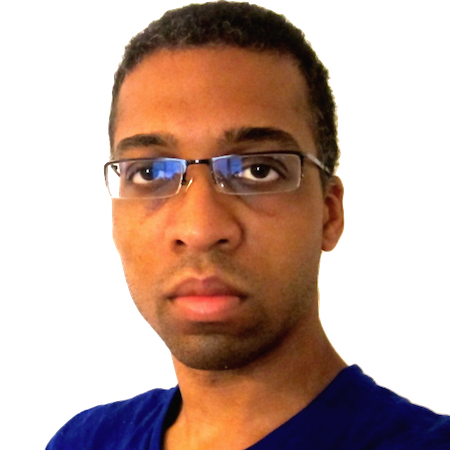
\includegraphics[width=0.8\linewidth]{general_figures/alvin}
    \column{.6\linewidth}

        \begin{block}{ {\bf \href{http://umiacs.umd.edu/~jbg//docs/2015_emnlp_rewrite.pdf}{Syntax-based Rewriting for Simultaneous Machine Translation}}}
He He, Alvin Grissom II, {\bf Jordan Boyd-Graber}, and Hal {Daum\'{e} III}.  \emph{Empirical Methods in Natural Language Processing}, 2015
        \end{block}

        \begin{block}{ {\bf \href{http://umiacs.umd.edu/~jbg/docs/2016_naacl_interpretese.pdf}{Interpretese vs. Translationese: The Uniqueness of Human Strategies in Simultaneous Interpretation}}}
He He, {\bf Jordan Boyd-Graber}, and Hal {Daum\'{e} III}.
\emph{North American Association for Computational Linguistics}, 2016
        \end{block}

  \end{columns}


\end{frame}

\begin{frame}{Simultaneous Interpretation is Hard!}

  \begin{columns}
    \column{.5\linewidth}
  \begin{itemize}
    \item Exhausting for humans
    \item Computers not trusted
    \item Differential strengths
    \item Same word-by-word characteristic
  \end{itemize}

  \column{.5\linewidth}
 \gfxs{computer-interpreter}{1.0}
 \end{columns}
\end{frame}


\begin{frame}

\makebox[\linewidth]{
\includegraphics[width=\paperwidth]{general_figures/blackbox}}
\only<2>{

\vspace{-5cm}
\begin{block}{Takeaways}
  \begin{itemize}
    \item ML should be interpretable
    \item We should measure interpretability
    \item Interpretability should reflect the world we want
  \end{itemize}
\end{block}

}
\end{frame}




\frame{

	\frametitle{Thanks}

        \begin{block}{Collaborators}
          \textsc{naqt}, Hal Daum\'e III (UMD), Leah Findlater (UMD), Kevin Seppi
          (BYU), Eric Ringger
        \end{block}

	\begin{columns}

	\column{.75\linewidth}
        \begin{block}{Funders}
        \begin{center}
          
\includegraphics[width=0.2\linewidth]{general_figures/nsf}
          
\includegraphics[width=0.2\linewidth]{general_figures/darpa}
          
\includegraphics[width=0.2\linewidth]{general_figures/arl}
          
\includegraphics[width=0.2\linewidth]{general_figures/iarpa}
       \end{center}
        \end{block}

	\column{.3\linewidth}
        \begin{block}{Supporters}
        	\gfxq{naqt}{1.0}
        \end{block}

        \end{columns}
}



\frame{

\begin{columns}

\column{.5\linewidth}

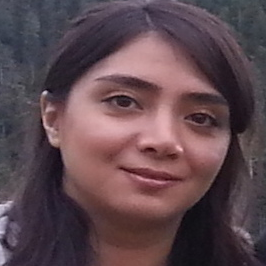
\includegraphics[width=.8\linewidth]{general_figures/forough}

\column{.5\linewidth}

\begin{block}{ALTO: Active Learning with Topic Overviews for Speeding Label Induction and Document Labeling}
Forough Poursabzi-Sangdeh, Jordan Boyd-Graber, Leah Findlater, and Kevin Seppi.  Association for Computational Linguistics, 2016.
\end{block}

\end{columns}

}



\fsi{interactive_topic_models/alto_interface}{}
\fsi{interactive_topic_models/alto_interface_highlight}{Direct users
  to document}



\fsi{interactive_topic_models/alto/user_talk_1}{ Active learning if time is short}
\fsi{interactive_topic_models/alto/user_talk_2}{ Better than status quo}
\fsi{interactive_topic_models/alto/user_talk_3}{ Active learning can
  help topic models }
\fsi{interactive_topic_models/alto/user_talk_4}{ Topic models help
  users understand the collection }
\fsi{interactive_topic_models/alto/user_talk_4}{ Moral: machines and
  humans together (if you let them) }

\begin{frame}[plain]
  \vspace{-2cm}
		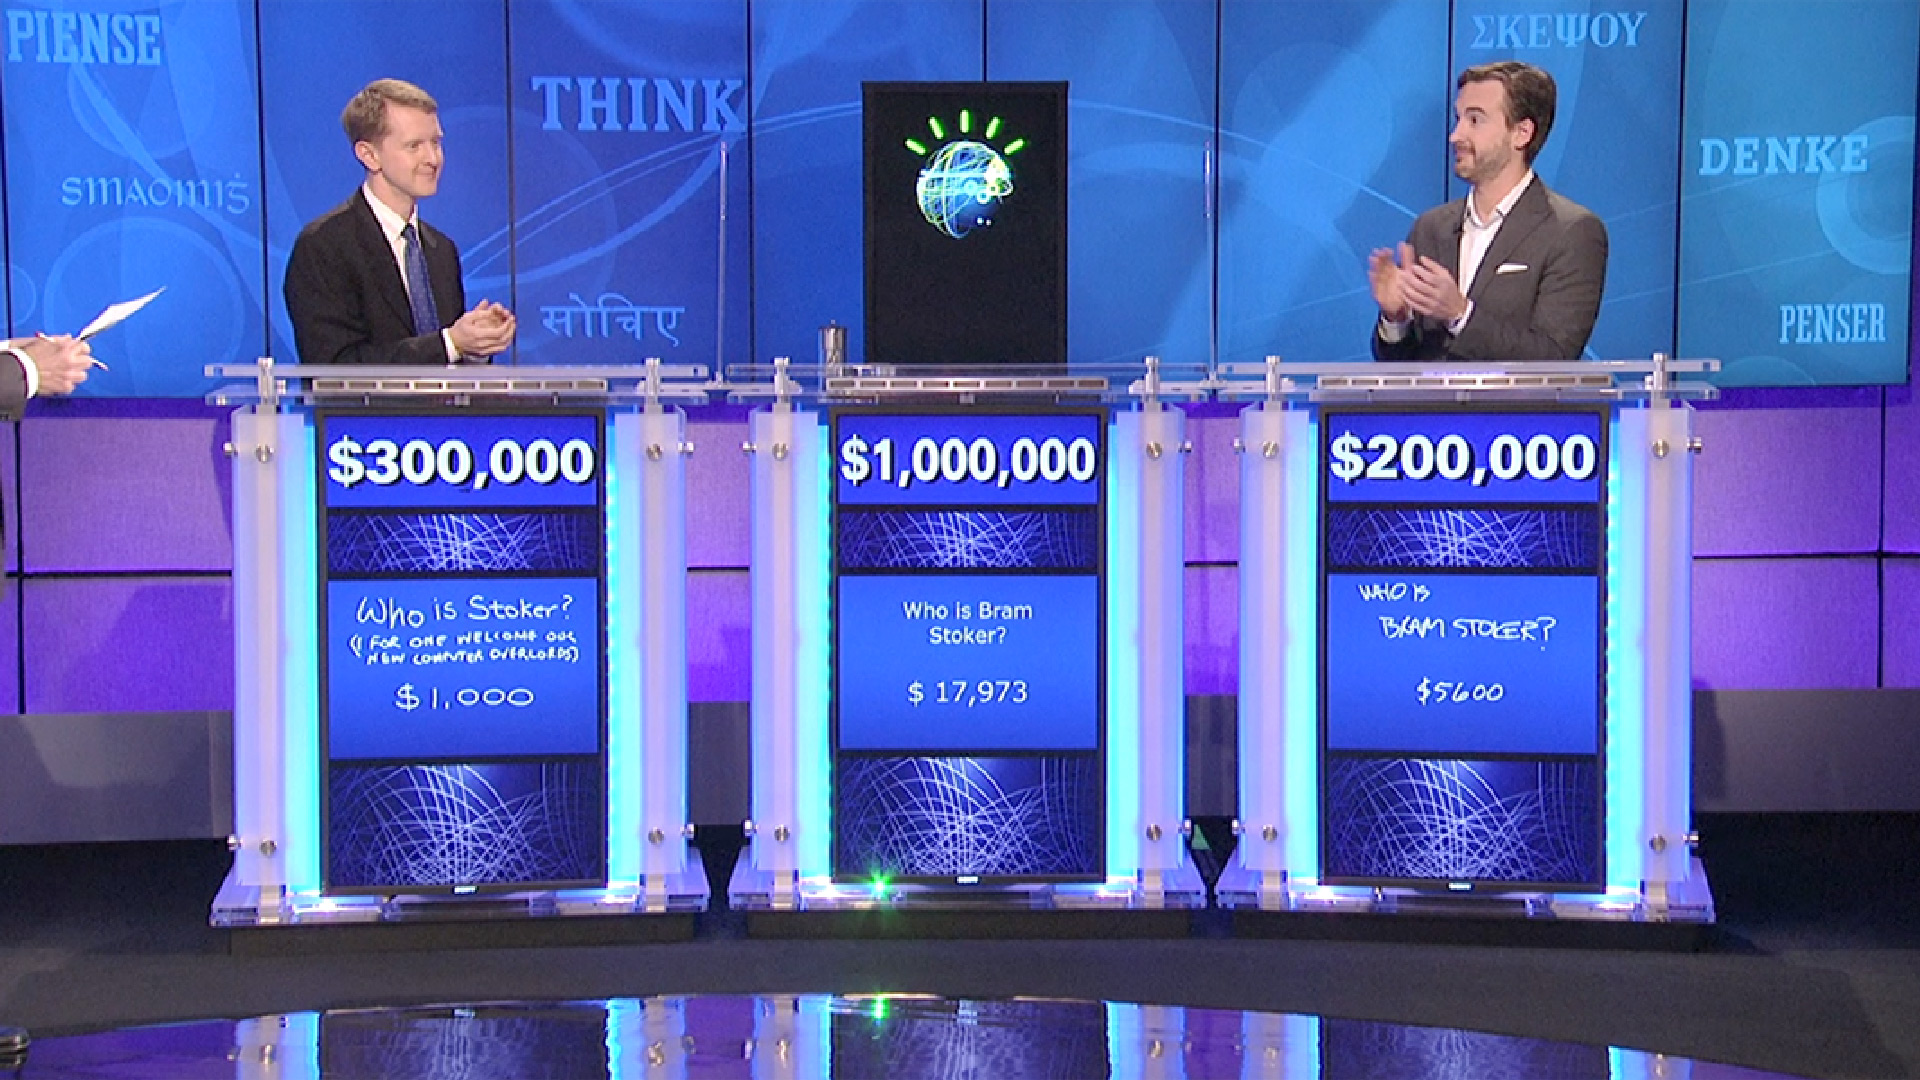
\includegraphics[width=1.0\linewidth]{qb/jeopardy}
                \pause
                \vspace{-8cm}
         \begin{block}{This is {\bf not} Jeopardy}
		\begin{itemize}
                        \item Jeopardy: must decide to answer {\bf once}, after
                          complete question
                        \item Quiz Bowl: decide after each word
		\end{itemize}

	\end{block}

\end{frame}


\frame{

\begin{columns}

\column{.5\linewidth}

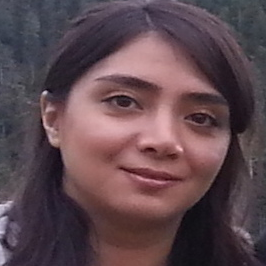
\includegraphics[width=.8\linewidth]{general_figures/forough}

\column{.5\linewidth}

\begin{block}{ALTO: Active Learning with Topic Overviews for Speeding Label Induction and Document Labeling}
Forough Poursabzi-Sangdeh, Jordan Boyd-Graber, Leah Findlater, and Kevin Seppi.  Association for Computational Linguistics, 2016.
\end{block}

\end{columns}

}

\fsi{interactive_topic_models/messy-desk}{Many Documents}

\fsi{interactive_topic_models/file-cabinet}{Sort into Categories}

\begin{frame}{Evaluation}

  \begin{itemize}
    \item User study
    \item 40 minutes
    \item Sort documents into categories
    \item What information / interface \alert<2>{helps best}
      \pause
      \pause
      \begin{itemize}
        \item Train a classifier on human examples
          \only<4->{\alert<4>{(don't tell them how many labels)}}
        \item Compare classifier labels to expert judgements
          \only<5->{\alert<5>{(purity)}}
\only<5>{
\begin{equation}
\mbox{purity}(\mathbf{U},\mathbf{G}) = \frac{1}{N}\sum\limits_{l} \max\limits_{j}|U_l \cap G_j|,
\end{equation}
}
      \end{itemize}
  \end{itemize}

\end{frame}

\begin{frame}{Which is more Useful?}

\only<1>{
  \begin{center}
    Who should drive?
  \end{center}
}


\only<2->{
\begin{columns}
  \column{.5\linewidth}
    \begin{block}{Active Learning}
      \begin{center}
        \includegraphics[width=.85\linewidth]{interactive_topic_models/active_learning}
      \end{center}
    \end{block}
  \column{.5\linewidth}
  \pause
    \begin{block}{Topic Models}
      \begin{center}
        \includegraphics[width=.475\linewidth]{interactive_topic_models/nyt_topics}
      \end{center}

    \end{block}


\end{columns}
}

\end{frame}

\fsi{interactive_topic_models/alto_interface}{}
\fsi{interactive_topic_models/alto_interface_highlight}{Direct users
  to document}



\fsi{interactive_topic_models/alto/user_talk_1}{ Active learning if time is short}
\fsi{interactive_topic_models/alto/user_talk_2}{ Better than status quo}
\fsi{interactive_topic_models/alto/user_talk_3}{ Active learning can
  help topic models }
\fsi{interactive_topic_models/alto/user_talk_4}{ Topic models help
  users understand the collection }
\fsi{interactive_topic_models/alto/user_talk_4}{ Moral: machines and
  humans together (if you let them) }



\begin{frame}{References}
\bibliographystyle{style/acl}
\tiny
\bibliography{bib/journal-full,bib/jbg,bib/hhe,bib/alvin,teaparty/vietan}
\end{frame}



\end{document}
